
%% This style is provided exclusively for the ICSE 2012 main conference,
%% ICSE 2012 co-located events, and ICSE 2012 workshops.

%% bare_conf_ICSE12.tex
%% V1.4
%% 2012-01-21
%%

%% This is a skeleton file demonstrating the use of IEEEtran.cls
%% (requires IEEEtran.cls version 1.7 or later) with an IEEE conference paper.
%%
%% Support sites:
%% http://www.michaelshell.org/tex/ieeetran/
%% http://www.ctan.org/tex-archive/macros/latex/contrib/IEEEtran/
%% and
%% http://www.ieee.org/

%%*************************************************************************
%% Legal Notice: 
%% This code is offered as-is without any warranty either expressed or
%% implied; without even the implied warranty of MERCHANTABILITY or
%% FITNESS FOR A PARTICULAR PURPOSE! 
%% User assumes all risk.
%% In no event shall IEEE or any contributor to this code be liable for
%% any damages or losses, including, but not limited to, incidental,
%% consequential, or any other damages, resulting from the use or misuse
%% of any information contained here.
%%
%% All comments are the opinions of their respective authors and are not
%% necessarily endorsed by the IEEE.
%%
%% This work is distributed under the LaTeX Project Public License (LPPL)
%% ( http://www.latex-project.org/ ) version 1.3, and may be freely used,
%% distributed and modified. A copy of the LPPL, version 1.3, is included
%% in the base LaTeX documentation of all distributions of LaTeX released
%% 2003/12/01 or later.
%% Retain all contribution notices and credits.
%% ** Modified files should be clearly indicated as such, including  **
%% ** renaming them and changing author support contact information. **
%%
%% File list of work: IEEEtran.cls, IEEEtran_HOWTO.pdf, bare_adv.tex,
%%                    bare_conf.tex, bare_jrnl.tex, bare_jrnl_compsoc.tex
%%*************************************************************************

% *** Authors should verify (and, if needed, correct) their LaTeX system  ***
% *** with the testflow diagnostic prior to trusting their LaTeX platform ***
% *** with production work. IEEE's font choices can trigger bugs that do  ***
% *** not appear when using other class files.                            ***
% The testflow support page is at:
% http://www.michaelshell.org/tex/testflow/



% Note that the a4paper option is mainly intended so that authors in
% countries using A4 can easily print to A4 and see how their papers will
% look in print - the typesetting of the document will not typically be
% affected with changes in paper size (but the bottom and side margins will).
% Use the testflow package mentioned above to verify correct handling of
% both paper sizes by the user's LaTeX system.
%
% Also note that the "draftcls" or "draftclsnofoot", not "draft", option
% should be used if it is desired that the figures are to be displayed in
% draft mode.
%
\documentclass[10pt, conference, compsocconf]{IEEEtran}
% Add the compsocconf option for Computer Society conferences.
%
% If IEEEtran.cls has not been installed into the LaTeX system files,
% manually specify the path to it like:
% \documentclass[conference]{../sty/IEEEtran}


\usepackage{balance}
\usepackage{float}

% Some very useful LaTeX packages include:
% (uncomment the ones you want to load)


% *** MISC UTILITY PACKAGES ***
%
%\usepackage{ifpdf}
% Heiko Oberdiek's ifpdf.sty is very useful if you need conditional
% compilation based on whether the output is pdf or dvi.
% usage:
% \ifpdf
%   % pdf code
% \else
%   % dvi code
% \fi
% The latest version of ifpdf.sty can be obtained from:
% http://www.ctan.org/tex-archive/macros/latex/contrib/oberdiek/
% Also, note that IEEEtran.cls V1.7 and later provides a builtin
% \ifCLASSINFOpdf conditional that works the same way.
% When switching from latex to pdflatex and vice-versa, the compiler may
% have to be run twice to clear warning/error messages.






% *** CITATION PACKAGES ***
%
%\usepackage{cite}
% cite.sty was written by Donald Arseneau
% V1.6 and later of IEEEtran pre-defines the format of the cite.sty package
% \cite{} output to follow that of IEEE. Loading the cite package will
% result in citation numbers being automatically sorted and properly
% "compressed/ranged". e.g., [1], [9], [2], [7], [5], [6] without using
% cite.sty will become [1], [2], [5]--[7], [9] using cite.sty. cite.sty's
% \cite will automatically add leading space, if needed. Use cite.sty's
% noadjust option (cite.sty V3.8 and later) if you want to turn this off.
% cite.sty is already installed on most LaTeX systems. Be sure and use
% version 4.0 (2003-05-27) and later if using hyperref.sty. cite.sty does
% not currently provide for hyperlinked citations.
% The latest version can be obtained at:
% http://www.ctan.org/tex-archive/macros/latex/contrib/cite/
% The documentation is contained in the cite.sty file itself.






% *** GRAPHICS RELATED PACKAGES ***
%
\ifCLASSINFOpdf
  \usepackage[pdftex]{graphicx}
  % declare the path(s) where your graphic files are
  \graphicspath{{../pdf/}{../jpeg/}}
  % and their extensions so you won't have to specify these with
  % every instance of \includegraphics
  \DeclareGraphicsExtensions{.pdf,.jpeg,.png}
\else
  % or other class option (dvipsone, dvipdf, if not using dvips). graphicx
  % will default to the driver specified in the system graphics.cfg if no
  % driver is specified.
  \usepackage[dvips]{graphicx}
  % declare the path(s) where your graphic files are
  \graphicspath{{../eps/}}
  % and their extensions so you won't have to specify these with
  % every instance of \includegraphics
  \DeclareGraphicsExtensions{.eps}
\fi
% graphicx was written by David Carlisle and Sebastian Rahtz. It is
% required if you want graphics, photos, etc. graphicx.sty is already
% installed on most LaTeX systems. The latest version and documentation can
% be obtained at: 
% http://www.ctan.org/tex-archive/macros/latex/required/graphics/
% Another good source of documentation is "Using Imported Graphics in
% LaTeX2e" by Keith Reckdahl which can be found as epslatex.ps or
% epslatex.pdf at: http://www.ctan.org/tex-archive/info/
%
% latex, and pdflatex in dvi mode, support graphics in encapsulated
% postscript (.eps) format. pdflatex in pdf mode supports graphics
% in .pdf, .jpeg, .png and .mps (metapost) formats. Users should ensure
% that all non-photo figures use a vector format (.eps, .pdf, .mps) and
% not a bitmapped formats (.jpeg, .png). IEEE frowns on bitmapped formats
% which can result in "jaggedy"/blurry rendering of lines and letters as
% well as large increases in file sizes.
%
% You can find documentation about the pdfTeX application at:
% http://www.tug.org/applications/pdftex





% *** MATH PACKAGES ***
%
%\usepackage[cmex10]{amsmath}
% A popular package from the American Mathematical Society that provides
% many useful and powerful commands for dealing with mathematics. If using
% it, be sure to load this package with the cmex10 option to ensure that
% only type 1 fonts will utilized at all point sizes. Without this option,
% it is possible that some math symbols, particularly those within
% footnotes, will be rendered in bitmap form which will result in a
% document that can not be IEEE Xplore compliant!
%
% Also, note that the amsmath package sets \interdisplaylinepenalty to 10000
% thus preventing page breaks from occurring within multiline equations. Use:
%\interdisplaylinepenalty=2500
% after loading amsmath to restore such page breaks as IEEEtran.cls normally
% does. amsmath.sty is already installed on most LaTeX systems. The latest
% version and documentation can be obtained at:
% http://www.ctan.org/tex-archive/macros/latex/required/amslatex/math/





% *** SPECIALIZED LIST PACKAGES ***
%
%\usepackage{algorithmic}
% algorithmic.sty was written by Peter Williams and Rogerio Brito.
% This package provides an algorithmic environment fo describing algorithms.
% You can use the algorithmic environment in-text or within a figure
% environment to provide for a floating algorithm. Do NOT use the algorithm
% floating environment provided by algorithm.sty (by the same authors) or
% algorithm2e.sty (by Christophe Fiorio) as IEEE does not use dedicated
% algorithm float types and packages that provide these will not provide
% correct IEEE style captions. The latest version and documentation of
% algorithmic.sty can be obtained at:
% http://www.ctan.org/tex-archive/macros/latex/contrib/algorithms/
% There is also a support site at:
% http://algorithms.berlios.de/index.html
% Also of interest may be the (relatively newer and more customizable)
% algorithmicx.sty package by Szasz Janos:
% http://www.ctan.org/tex-archive/macros/latex/contrib/algorithmicx/




% *** ALIGNMENT PACKAGES ***
%
%\usepackage{array}
% Frank Mittelbach's and David Carlisle's array.sty patches and improves
% the standard LaTeX2e array and tabular environments to provide better
% appearance and additional user controls. As the default LaTeX2e table
% generation code is lacking to the point of almost being broken with
% respect to the quality of the end results, all users are strongly
% advised to use an enhanced (at the very least that provided by array.sty)
% set of table tools. array.sty is already installed on most systems. The
% latest version and documentation can be obtained at:
% http://www.ctan.org/tex-archive/macros/latex/required/tools/


%\usepackage{mdwmath}
%\usepackage{mdwtab}
% Also highly recommended is Mark Wooding's extremely powerful MDW tools,
% especially mdwmath.sty and mdwtab.sty which are used to format equations
% and tables, respectively. The MDWtools set is already installed on most
% LaTeX systems. The lastest version and documentation is available at:
% http://www.ctan.org/tex-archive/macros/latex/contrib/mdwtools/


% IEEEtran contains the IEEEeqnarray family of commands that can be used to
% generate multiline equations as well as matrices, tables, etc., of high
% quality.


%\usepackage{eqparbox}
% Also of notable interest is Scott Pakin's eqparbox package for creating
% (automatically sized) equal width boxes - aka "natural width parboxes".
% Available at:
% http://www.ctan.org/tex-archive/macros/latex/contrib/eqparbox/





% *** SUBFIGURE PACKAGES ***
%\usepackage[tight,footnotesize]{subfigure}
% subfigure.sty was written by Steven Douglas Cochran. This package makes it
% easy to put subfigures in your figures. e.g., "Figure 1a and 1b". For IEEE
% work, it is a good idea to load it with the tight package option to reduce
% the amount of white space around the subfigures. subfigure.sty is already
% installed on most LaTeX systems. The latest version and documentation can
% be obtained at:
% http://www.ctan.org/tex-archive/obsolete/macros/latex/contrib/subfigure/
% subfigure.sty has been superceeded by subfig.sty.



%\usepackage[caption=false]{caption}
%\usepackage[font=footnotesize]{subfig}
% subfig.sty, also written by Steven Douglas Cochran, is the modern
% replacement for subfigure.sty. However, subfig.sty requires and
% automatically loads Axel Sommerfeldt's caption.sty which will override
% IEEEtran.cls handling of captions and this will result in nonIEEE style
% figure/table captions. To prevent this problem, be sure and preload
% caption.sty with its "caption=false" package option. This is will preserve
% IEEEtran.cls handing of captions. Version 1.3 (2005/06/28) and later 
% (recommended due to many improvements over 1.2) of subfig.sty supports
% the caption=false option directly:
%\usepackage[caption=false,font=footnotesize]{subfig}
%
% The latest version and documentation can be obtained at:
% http://www.ctan.org/tex-archive/macros/latex/contrib/subfig/
% The latest version and documentation of caption.sty can be obtained at:
% http://www.ctan.org/tex-archive/macros/latex/contrib/caption/




% *** FLOAT PACKAGES ***
%
%\usepackage{fixltx2e}
% fixltx2e, the successor to the earlier fix2col.sty, was written by
% Frank Mittelbach and David Carlisle. This package corrects a few problems
% in the LaTeX2e kernel, the most notable of which is that in current
% LaTeX2e releases, the ordering of single and double column floats is not
% guaranteed to be preserved. Thus, an unpatched LaTeX2e can allow a
% single column figure to be placed prior to an earlier double column
% figure. The latest version and documentation can be found at:
% http://www.ctan.org/tex-archive/macros/latex/base/



%\usepackage{stfloats}
% stfloats.sty was written by Sigitas Tolusis. This package gives LaTeX2e
% the ability to do double column floats at the bottom of the page as well
% as the top. (e.g., "\begin{figure*}[!b]" is not normally possible in
% LaTeX2e). It also provides a command:
%\fnbelowfloat
% to enable the placement of footnotes below bottom floats (the standard
% LaTeX2e kernel puts them above bottom floats). This is an invasive package
% which rewrites many portions of the LaTeX2e float routines. It may not work
% with other packages that modify the LaTeX2e float routines. The latest
% version and documentation can be obtained at:
% http://www.ctan.org/tex-archive/macros/latex/contrib/sttools/
% Documentation is contained in the stfloats.sty comments as well as in the
% presfull.pdf file. Do not use the stfloats baselinefloat ability as IEEE
% does not allow \baselineskip to stretch. Authors submitting work to the
% IEEE should note that IEEE rarely uses double column equations and
% that authors should try to avoid such use. Do not be tempted to use the
% cuted.sty or midfloat.sty packages (also by Sigitas Tolusis) as IEEE does
% not format its papers in such ways.





% *** PDF, URL AND HYPERLINK PACKAGES ***
%
%\usepackage{url}
% url.sty was written by Donald Arseneau. It provides better support for
% handling and breaking URLs. url.sty is already installed on most LaTeX
% systems. The latest version can be obtained at:
% http://www.ctan.org/tex-archive/macros/latex/contrib/misc/
% Read the url.sty source comments for usage information. Basically,
% \url{my_url_here}.





% *** Do not adjust lengths that control margins, column widths, etc. ***
% *** Do not use packages that alter fonts (such as pslatex).         ***
% There should be no need to do such things with IEEEtran.cls V1.6 and later.
% (Unless specifically asked to do so by the journal or conference you plan
% to submit to, of course. )


% correct bad hyphenation here
\hyphenation{op-tical net-works semi-conduc-tor}


\begin{document}
%
% paper title
% can use linebreaks \\ within to get better formatting as desired
\title{Mining the Temporal Evolution of the Android Bug Reporting
  Community \\ via Sliding Windows}


% author names and affiliations
% use a multiple column layout for up to two different
% affiliations

\author{\IEEEauthorblockN{\quad \quad \quad \quad \quad Feng Jiang, Jiemin Wang, Abram Hindle, Mario A. Nascimento}
\IEEEauthorblockA{\quad \quad \quad \quad \quad Department of Computing Science\\
\quad \quad \quad \quad \quad University of Alberta\\
\quad \quad \quad \quad \quad Edmonton, Alberta, Canada\\
\quad \quad \quad \quad \quad \{fjiang2, jiemin2, abram.hindle, mario.nascimento\}@ualberta.ca}
\and

}

% conference papers do not typically use \thanks and this command
% is locked out in conference mode. If really needed, such as for
% the acknowledgment of grants, issue a \IEEEoverridecommandlockouts
% after \documentclass

% for over three affiliations, or if they all won't fit within the width
% of the page, use this alternative format:
% 
%\author{\IEEEauthorblockN{Michael Shell\IEEEauthorrefmark{1},
%Homer Simpson\IEEEauthorrefmark{2},
%James Kirk\IEEEauthorrefmark{3}, 
%Montgomery Scott\IEEEauthorrefmark{3} and
%Eldon Tyrell\IEEEauthorrefmark{4}}
%\IEEEauthorblockA{\IEEEauthorrefmark{1}School of Electrical and Computer Engineering\\
%Georgia Institute of Technology,
%Atlanta, Georgia 30332--0250\\ Email: see http://www.michaelshell.org/contact.html}
%\IEEEauthorblockA{\IEEEauthorrefmark{2}Twentieth Century Fox, Springfield, USA\\
%Email: homer@thesimpsons.com}
%\IEEEauthorblockA{\IEEEauthorrefmark{3}Starfleet Academy, San Francisco, California 96678-2391\\
%Telephone: (800) 555--1212, Fax: (888) 555--1212}
%\IEEEauthorblockA{\IEEEauthorrefmark{4}Tyrell Inc., 123 Replicant Street, Los Angeles, California 90210--4321}}




% use for special paper notices
%\IEEEspecialpapernotice{(Invited Paper)}




% make the title area
\maketitle


\begin{abstract}
% need to be expanded !!!

The open source development community consists of both paid and volunteer
developers as well as new and experienced users.
Previous work has applied social network analysis (SNA) to open source
communities and has demonstrated value in expertise discovery and
triaging. 
One problem with applying SNA is that time period of evaluation is
often important. Too large a window and the most frequent participants
drown out the impact of less frequent participants, too small a window
produces a local analysis irrelevant to the global view of the
community.
In this paper we provide a method of aggregating, analyzing, and visualizing local
interactions (small time periods) of bug reporting participants by
using the SNA measure of betweeness centrality to indicate participant
activity. 
In particular we mined the Android bug repository by producing 
social networks from the 30-day windows of bug reports, each sliding
over by day.
Within Android, we find and validate three patterns of participant
behaviour based on their local centrality.
In this paper we provide a method of analyzing centrality of bug
report participants both locally and globally and we use it to provide
a thorough case study of the bug reporter activity within the Android
bug repository.

\end{abstract}

\begin{IEEEkeywords}
mining software repository; social network analysis; sliding windows

\end{IEEEkeywords}


% For peer review papers, you can put extra information on the cover
% page as needed:
% \ifCLASSOPTIONpeerreview
% \begin{center} \bfseries EDICS Category: 3-BBND \end{center}
% \fi
%
% For peerreview papers, this IEEEtran command inserts a page break and
% creates the second title. It will be ignored for other modes.
\IEEEpeerreviewmaketitle



\section{Introduction}
% two columns !!!

\label{introduction}
% no \IEEEPARstart
An important aspect of applying Social Network Analysis (SNA) to
software development teams is studying the development communities,
since the interaction in the communities records the activities of
each participant and the communication among them
\cite{ICSEsocio:meneely}. 
The activities are supposed to reflect the project development process
or even the project structure.


On the other hand, although with good management of development
process, it is still difficult to view the structure of the whole
community. 
For example, for open source software, developers are usually composed
of volunteers and do not form into structural organizations
\cite{ACM:chris}. 
Open source projects usually do not have central control and plans
\cite{AMCIS:Freeh}. 
Some tasks are chosen by developers rather than being assigned
\cite{ACM:ashish}. 
It is also true for some big and complicated projects, which cover
huge varieties of technique issues. 
Developers of such projects would be organized into departments, but
one single department could still be working on problems related with
multiple technique areas. 
In this case, even with organization, people's activities are not
necessarily in accordance with the departments they belong to.
For this matter, if the SNA could reflect developers' activities and
relations which we can trust to some extent, it would significantly
help the open source project management. 
We would be able to find potential groups of developers who work on
the same technical areas, so that we can assign tasks on
technical-group level. 
Besides, with better sight about developers, we could easily look for
experts when needed as well.


%In this paper, we studied the Android bug community. The Android development contains both the systems or the sdks and the apps; it covers varieties of technique topics, and at the same time, developers are not organized statically as the very standard commercial software. The Android development comprises participants from different vanders, for example, some are from Motorola, some are from HTC, or Samsung, etc, and thus it should be interesting and worthwhile to study the Android community and see how well it could relate to the development facts. 

In the case of Android bug reporting repository provided by 2012 MSR
Mining Challenge \cite{DATA:msr}, a reporter would report a bug, which
might attract comments discussing the reasons, the solutions, the bug
histories, etc. 
The bug reporting community members are comprised of both bug
reporters and commenters who could be either Android developers or
Android users who are often fans of Android. 
From the perspective of the bug repository, there is actually no
obvious boundary between a user and a developer. 
All of them are participating in making contributions to the project,
and they form the networks when acting as reporters and making
comments on bugs. 
We call both of the groups bug participants in this paper.

In order to use SNA, we pose that each node of the network represents
one bug participant and each edge represents the connection between
two participants who have communicated on the same bug. 
The edge weights indicate the amount that two persons communicate with
each other. 
We will discuss the detailed characteristics of our network graphs in
Section ~\ref{methodology}.


We use betweenness centrality to quantify the importance of a
participant in the community \cite{ICSEsocio:la}. 
Further explanation about the betweenness centrality will be
introduced in Section ~\ref{methodology}. 
The betweenness centrality could reveal two aspects of a participant
in a community network: 1) the quantity of bug reports (which attract
at least one comment) or comments they have made and 2) the importance
of the content of their reports or comments. 
When people have high betweenness, they might have: 1) reported
quantities of bugs with at least one comment on them, 2) made lots of
comments, 3) reported a very critical bug, 4) or made a very
interesting comment which attracts comments from other participants.


Previous work which applied SNA to software development has been
introduced such as mining email archives and mining defect tracking
systems \cite{MSR:christ} \cite{ACM:ashish} \cite{OSD:yasu}. 
Similarly, we built our SNA on bug reporting repository, which
includes both bug reports and comments, and looked into the Android
bug community based on the participants' activities and discussions.


However, the previous work applied their SNA on the entire project
lifetime such that only a single community network was constructed. 
In this case, the results would only reflect a static view, but ignore
the trends and changing patterns of the community structures and the
participants' social characters. 
Thus, in this paper, we adopt the time windowed method so that we are
able to analyze the changes along the time line. 
We choose a period of 30 days as a window, slid one-day each time; we
make the network analysis for each window \cite{ICSMwindowed:hindle}. 
Moreover, by sliding one day, each pair of adjacent windows would have
an overlap, which results in smoother trends, and more importantly,
helps to maintain context. 
Other benefits provided by time windowed analysis is that it could
give a more accurate and nuanced view of the data
\cite{ICSEsocio:meneely} \cite{ICSMwindowed:hindle}. 
Locally central participants then would not be \textquotedblleft
drowned out\textquotedblright. 


Further, as mentioned above, when applying SNA to study the software
community, we expect a match between the hypothesis we made from the
mining results and the facts in real development process. 
To validate our hypothesis, we inspect the Android release
history\footnote[1]{Android release history:
  http://developer.android.com/sdk/index.html} and the Android changes
repository, both of which reflect the real development activities.
 We study the change records authored by bug participants (those who
 have submissions in the changes repository) to get the technique
 specialties and the type of tasks they were working on. 
The participants we selected are those who ever show high betweenness
centrality or have characterized activity patterns along the time
line. 
By inspecting the Android release history, we get the contents of each
major or minor releases. 
More details about the validation would be explained in Section
\ref{validation}.
 

In summary, in this paper, we use SNA to study the activities of bug
participants based on the Android bug reports and comments
repository. 
We apply the sliding time window method to get smoother change trends
along the time line. 
With these mining results, we seek to analyze bug participants'
interactions, activity trends and patterns. 
We then demonstrate our analysis results via answering the following
interesting questions from both local and global views.


Globally:

RQ1. How does the number of active bug participants change over time? Why?

RQ2. How does the betweenness centrality of a participant change over
time? What are the reasons if they have a certain activity pattern?


Locally:

RQ3. Are there special time ranges that participants are more/less
active or central than normal? Why?


RQ4. What are the possible scenarios for a very sharp change of the
participants' centrality?


The rest of our paper is organized as follows. 
Section \ref{background} introduces basic concepts and techniques we
used in this study. 
The specific steps and the methodology would be discussed in Section
\ref{methodology}. 
Section \ref{results} describes the details of our mining results. 
The analysis of the results and its corresponding validation is
provided in Section \ref{validation}. 
Section \ref{limitation} presents the limitations of our mining
process and Section \ref{conclusion} summarizes the paper and
discusses the future work.

%%%%%%%%%%%%%%4. What are the possible scenarios for the very sharp change in the participants' centrality?

% You must have at least 2 lines in the paragraph with the drop letter
% (should never be an issue)
\begin{figure}[!t]
\centerline{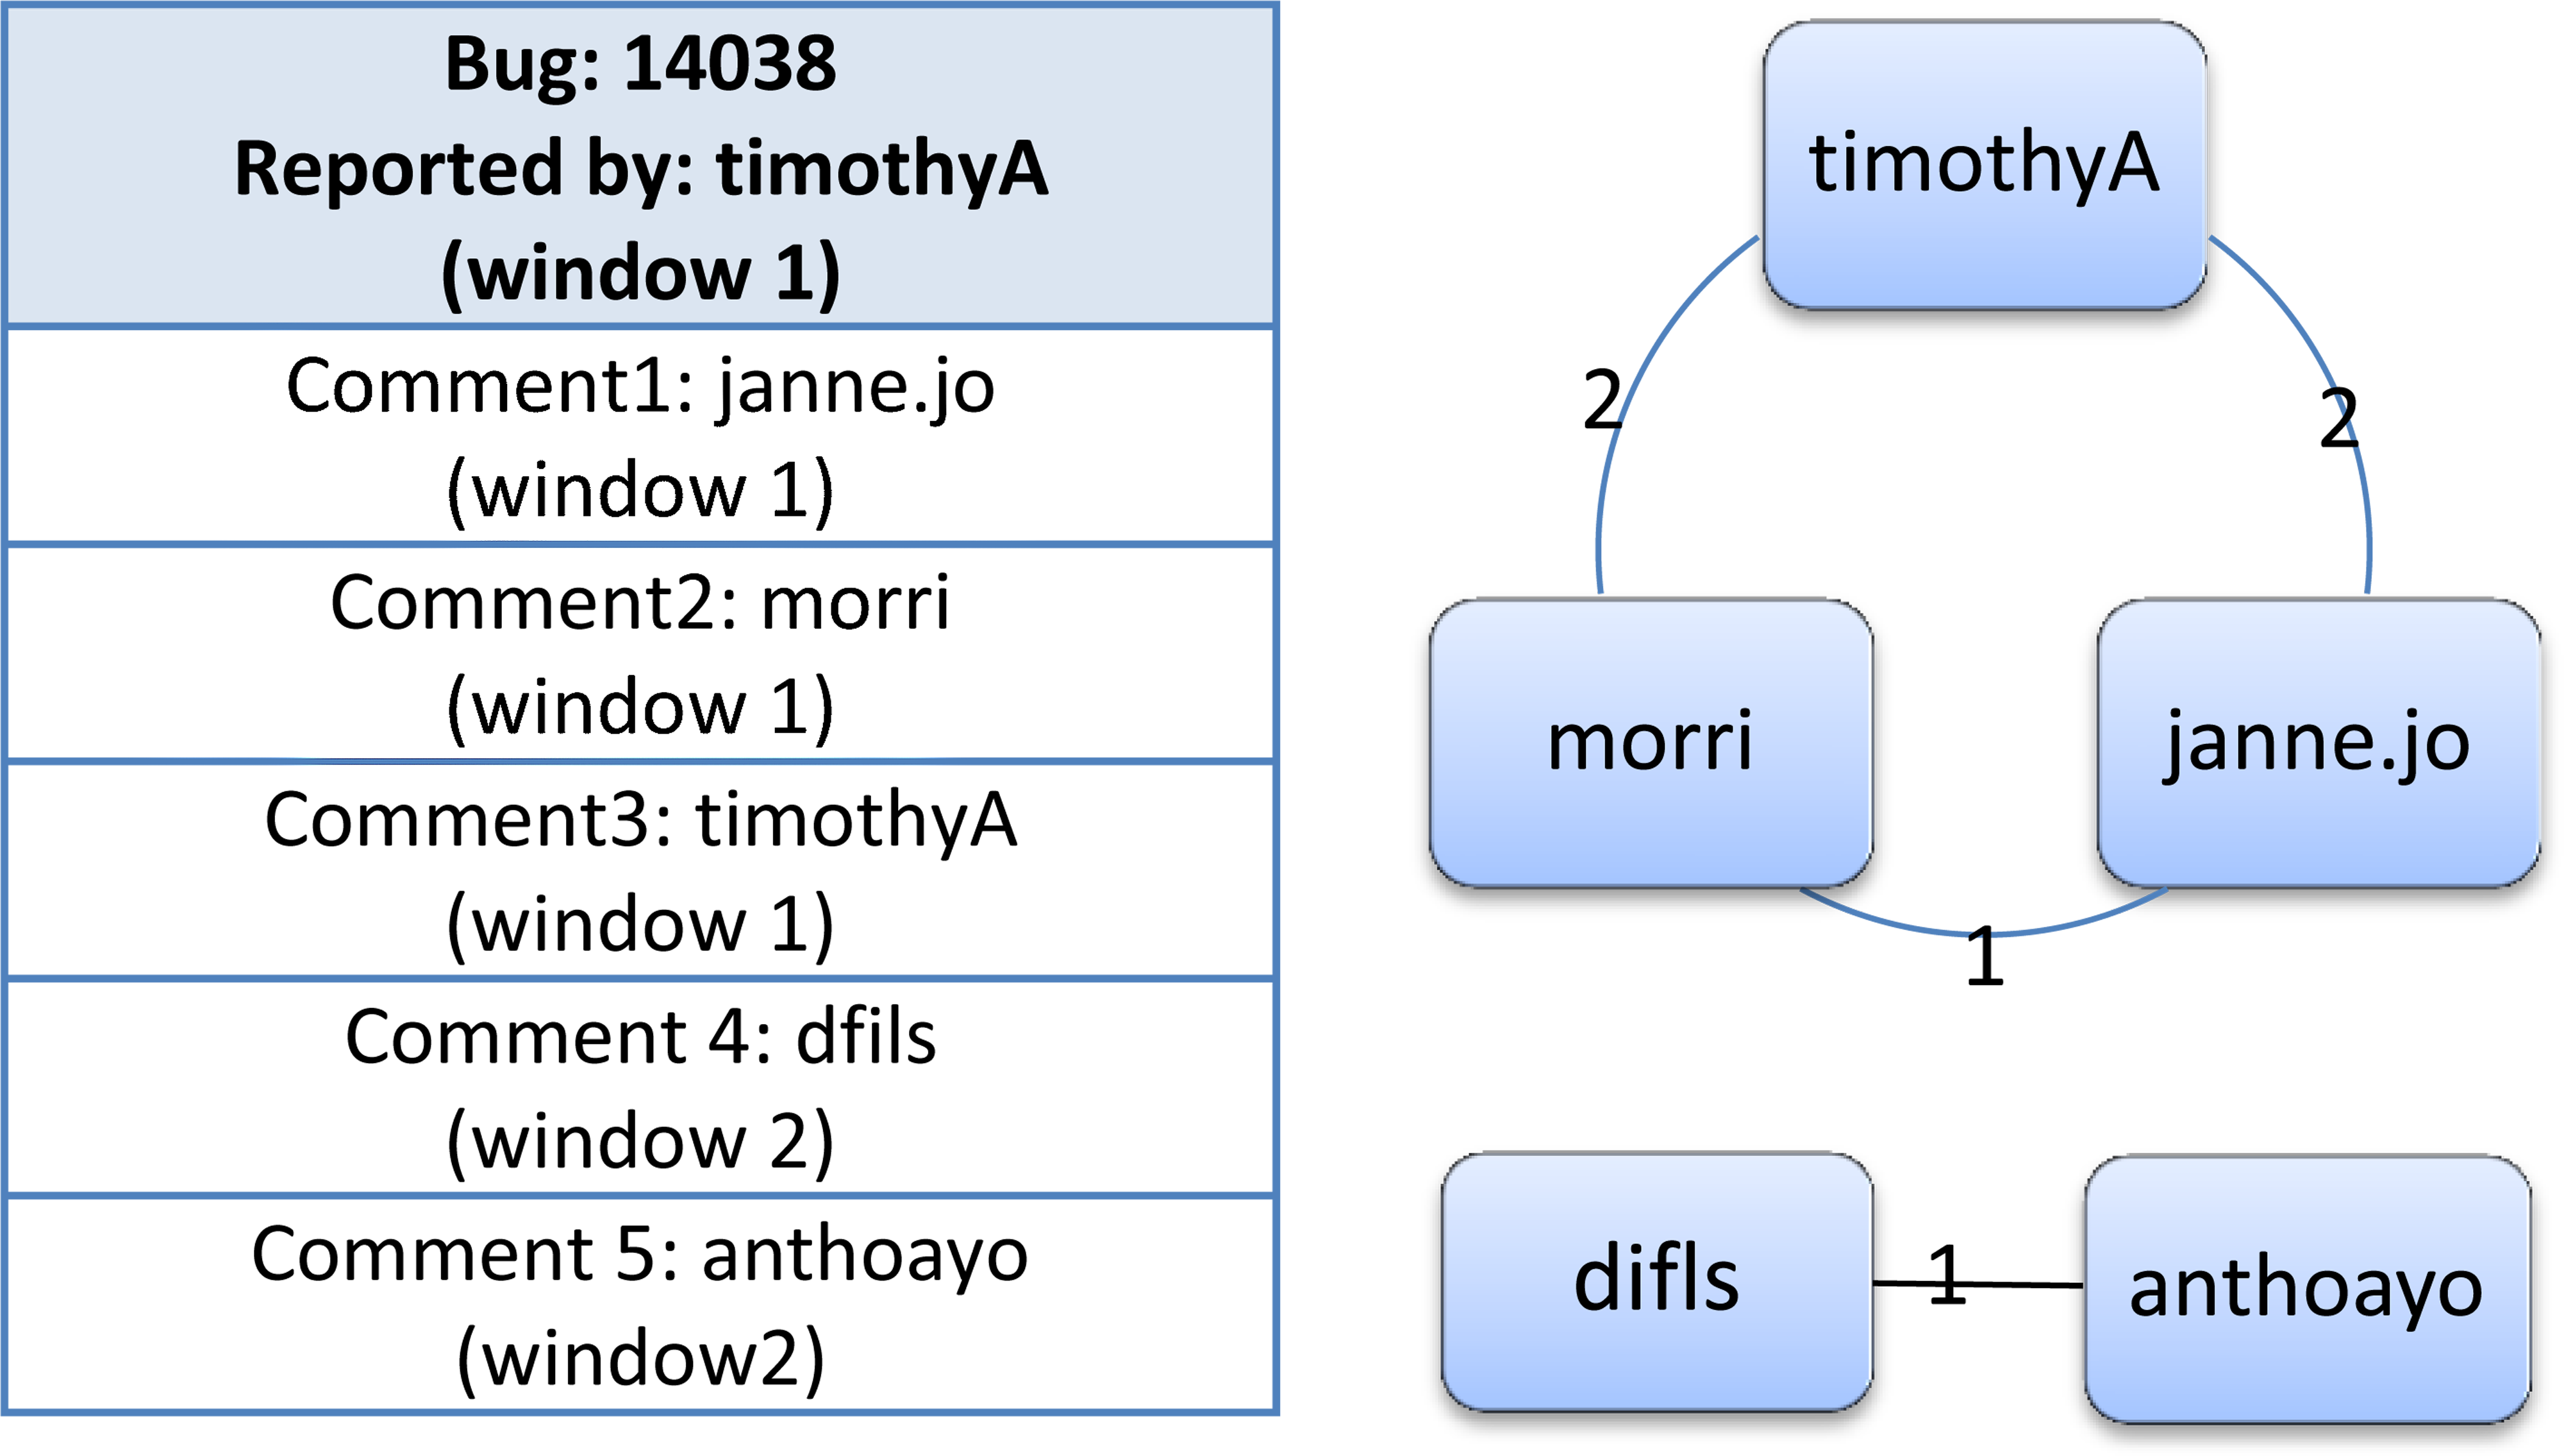
\includegraphics[width=2.6in,height = 3.8cm]{graph.png}
\label{graph}}
\caption{An example: bug 14038 is reported by timothyA, and there are
  five comments on this bug. 
When time window applied, comments are plotted into two windows, and
the bug report of this example forms two networks with the weight
noted on their edges}

\end{figure}

\section{Background}
\label{background}
% talk about window, overlap, cluster 
% need to take up 2 columns
\subsection{Betweenness}

The betweenness\footnote[2]{Introduction to centralities: http://en.wikipedia.org/wiki/Centrality} of a vertex is the number of geodesic paths in a graph that includes this vertex; the geodesic path is defined as the shortest path which has the minimum weight between two nodes. 
Defined by Freeman, the betweenness can be represented as:

\begin{equation} 
\sum_{i=1}^{j-1}\sum_{j=1}^{n}\frac{g_{ij}(p_k)}{g_{ij}}, i\neq j \neq k
\end{equation}

where $p_k$ is a vertex of the graph, $n$ is the total number of vertices, $i$ and $j$ are vertices other than $p_k$, $g_{ij}$ is the number of geodesic paths between vertex $i$ and $j$, and $g_{ij}(p_k)$ is the number of geodesic paths that include $p_k$.

It is used as a measurement of a person's importance in a network. A person would be regarded as central if they are on the geodesic path between two other persons. As proposed by Freeman, if a person locates on the geodesic path between two other persons, they become the key person who connects the others. That is, the more a person connects to the other people in a network, the more important or central they are \cite{BOOK:han}.

In our work, we normalize the betweenness centrality values with the number of node pairs to eliminate the effect of different sizes of the networks.

Compared with simply counting the total number of comments or total bug reports of a participant, betweenness acts better to reflect the interactions among people. For example, when a person reports lots of bugs but none of them attract any comment, it is very likely that their bug reports are not interesting or important. In this case, if we merely counted the number of their reports or comments, we would possibly increase their importance in the network artificially. Therefore, we choose to use betweenness centrality to eliminate this unfair counting \cite{ICSEsocio:la}.

\subsection{Overlapping Time Windowing}

Compared to the approaches in other papers which produce results on the entire time line chosen for the SNA, windowed analysis is to window the data by a period of time and perform the analysis within each window. With this approach, in addition to being able to overview the participants' relations in a social network, we can also study the changes or trends of their social activity \cite{ICSMwindowed:hindle}. 

Moreover, time windowing analysis could give a more accurate and nuanced view of the data \cite{ICSEsocio:meneely} \cite{ICSMwindowed:hindle}, as locally central participants would not be \textquotedblleft drowned out\textquotedblright. For instance, if a person participated in lots of bug reports and bug comments during one month from January 1st to January 30th, 2010, within this window, they would be one of the most central people with a high betweenness. However, if they never appeared except for that month. Globally they have low betweenness and would not be claimed as central, though in a local window they have played a vital role. 

Another point is that, comments on the same bug might not be temporally relevant \cite{Springer:kidane} \cite{Procedia:ibaa} so that a global time analysis would not make much sense in this case.

Furthermore, in this paper, we slide the windows by one day and there is an overlap between two adjacent windows. For two adjacent windows $A$ and $B$, $B$ starts on the second day of $A$, and they would have an overlapping of 29 days. Normally, windows could be either overlapped or not. We choose to use the overlapping window because the overlapping would smooth the trends and maintain the context. If there is a very sharp drop on values of a certain participant, the overlapping windows would give an insider's view of the change and what was happening.

\subsection{Clustering}
In order to perceive clusters and interactions, we clustered the bug participants by their betweenness centrality distribution along the time line. K-means is one of the most popular clustering methods. We choose to use K-means with Cosine distance since from the experiments, data clustered by K-means with Cosine distance gives a better view than K-means with Euclidean distance. Cosine distance calculates the similarity between each pair of data and Euclidean distance focuses on the magnitude of data. The Cosine distance between two vectors could be defined as,

\begin{equation}
Cosine\_dist(A,B) = 1-\frac{A\cdot B}{\Arrowvert A \Arrowvert \Arrowvert B \Arrowvert}
\end{equation}

where A and B are two vectors, $\{\cdot\}$ represents the inner dot operation and $\Arrowvert \cdot \Arrowvert$ indicates the module of the vector. With clustering, data with similar properties would be grouped together so that bug participants with similar activity patterns would also be grouped together. 

\section{Methodology}
% why window 7 days? clusters.
% take up 3 columns
\label{methodology}
\subsection{Data}
With the provided Android bug repository and the Android changes repository from the MSR challenge, we converted the XML format data to a database for efficient analysis using Microsoft SQL Server Business Intelligence. Our analysis focuses on the bug records of the previous two years from January 1st 2010 to December 4th 2011 since people during these two years are more active than the other years and the activities are representative, as showed in Figure 2. The data we used covers 14,432 out of 20,169 total bug records and 46,806 out of 67,730 total bug comments. Related to these bug and comment records, there are 30,969 people who have either reported a bug or made comments on a bug.

The bug and comment records are grouped into 30-day windows sliding by 1 day. The strategy of taking 30 days as a window and sliding by 1 day would be discussed in detail in Section \ref{methodology}. With this windowing strategy, we extracted 673 windows in total from the records of bug communities, despite of the data not provided after December 4th, 2011.

In addition, we make use of the data from Android changes repository to validate the mining results. The \textquotedblleft project\textquotedblright \ and the \textquotedblleft target\textquotedblright \ schema record all the submitted files from the developers, from which the actual behaviours could be identified.

\begin{figure*}[ht]
\centering
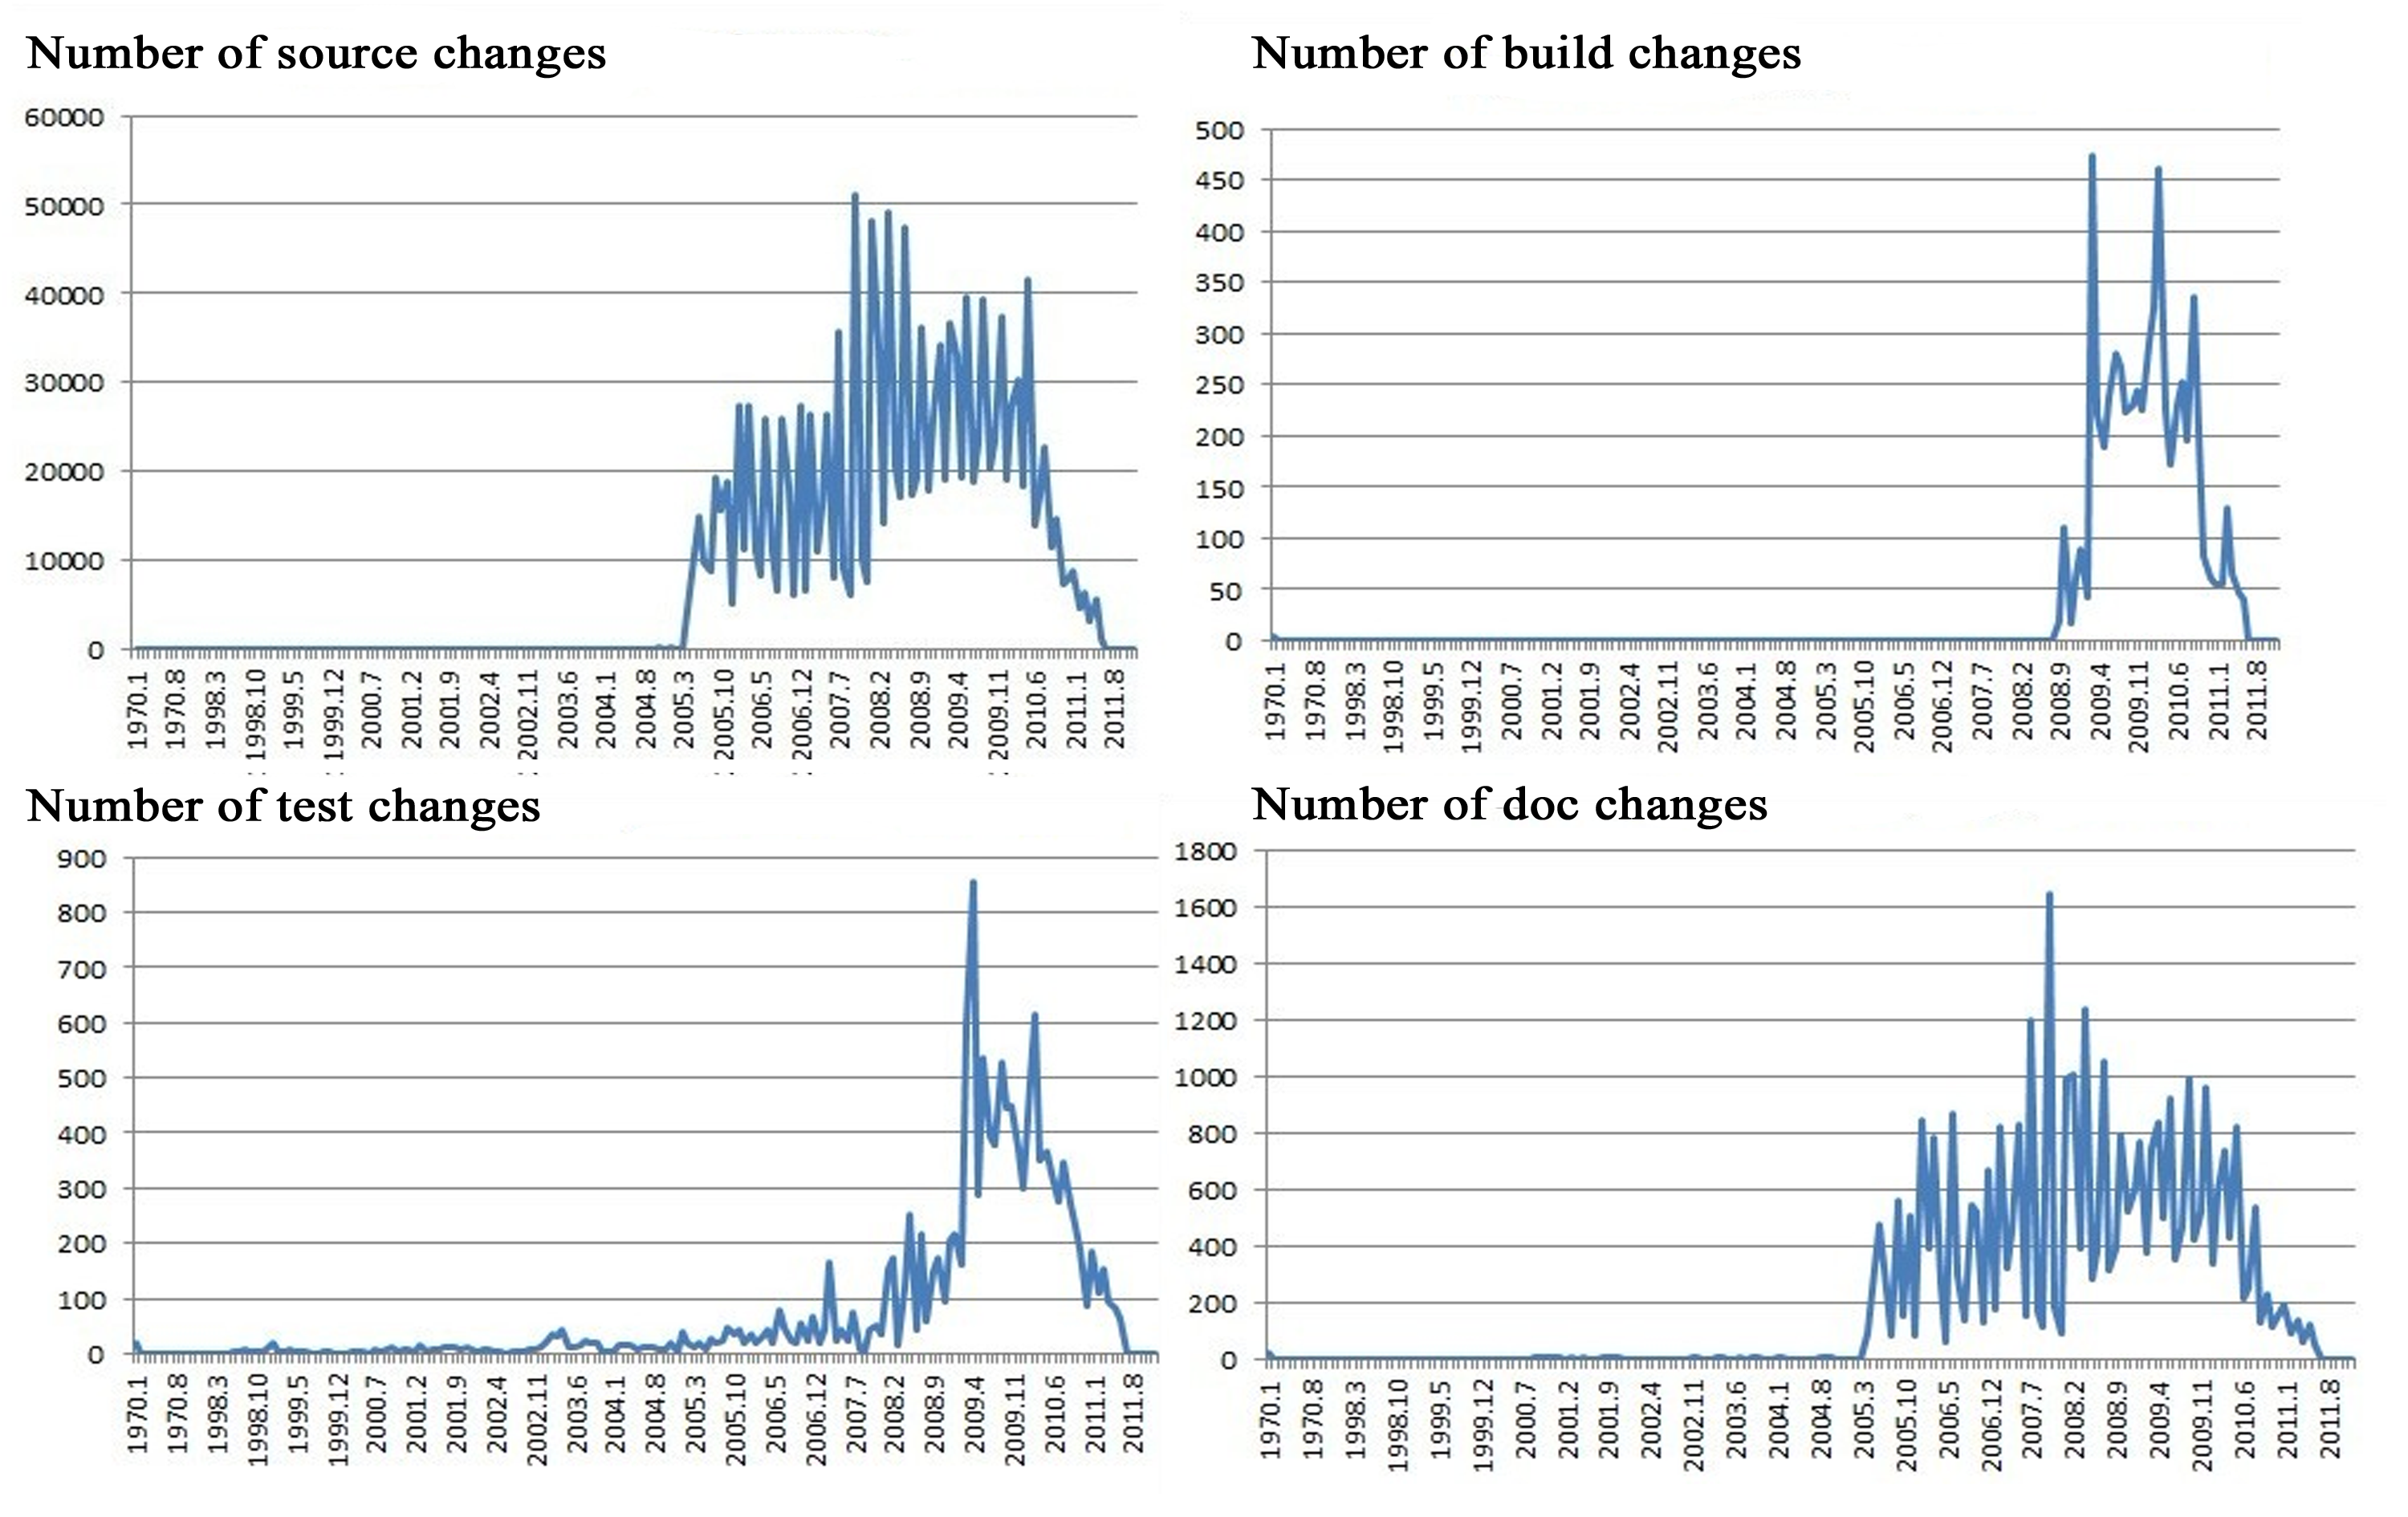
\includegraphics[width=13cm]{2010-2011.png}
\label{2010-2011}
\caption{Number of source files, build files, test files, and documentations submitted along the time line of the entire bug reports repository. The horizontal axis represents the time.}
\end{figure*}


\subsection{Methodology}
We windowed the data based on the time series and constructed networks indicating the relations among the participants within each specific window. Then, we calculated the betweenness centrality of each participant and drew the final graph. The steps of our methodology are explained as following:

\textbf{Step 1: Pruning the data.} We pruned the records of the reporters and commenters into pure name format, which are originally recorded in semi-anonymous email formats in the XML repository dump. For example, given the original email address which is represented by \textquotedblleft mathias....@gmail.com\textquotedblright, we truncate the string starting from \textquotedblleft ....\textquotedblright \ and keep the front part \textquotedblleft mathias\textquotedblright \ at the beginning as the name of the reporter or commenter. This strategy could lead to name aliasing problem, especially for common names or email addresses starting at just a simple letter like \textquotedblleft e....@gmail.com\textquotedblright. It is difficult or even impossible to eliminate the influence from this problem. Hence, we focus on the behaviour of normal cases, which means the cases where the names are less common and less ambiguous.

\textbf{Step 2: Windowing the records.} We windowed the data into periods of 30 days with a 29-day overlap. The reason for taking 30 days as a window is that from the extracted data, 30 days is a reasonable time period which contains enough changing information and at the same time excludes too much detail. In addition, sliding the next window by 1 day from the current one could result in smoother trends. We have compared it with our previous result from sliding by 7 days, the participants' arising and vanishing in the bug community could be described more gradually and smoothly by sliding only 1 day. Therefore, we choose to slide windows by 1 day to get better analysis results.

\textbf{Step 3: Establishing the network.} We made a SNA sliding window tool with Java and the JUNG Graph Framework, which read bug and comment records from the database and established social networks.

The nodes of the network represent participants who have either reported some bugs or made comments on bugs. The edges represent connections between two nodes. Besides, all the edges are weighted. For a certain bug within a selected time window, whenever a person makes a comment on this bug, the edge between the bug commenter and the bug reporter would get weight plus one, as well as the edges linking to the participants who previously make comments on this bug. Bug reports or comments in different windows would have separate network graph for their reporters or commenters. An example in Figure 1 indicates how the weighted network graph is built.

\textbf{Step 4: Calculating the centrality.} We calculated the betweenness centrality with JUNG, and normalized the centrality by dividing (n-1)(n-2)/2, which is the number of node pairs excluding the current node. We then get a list of all the bug participants and their betweenness centrality values for the total 673 overlapping windows.

\textbf{Step 5: Extracting the participants.} We removed the participants with betweenness centrality value 0, who might have either reported a bug/bugs with no comments, or made the only comment of a bug so that no other participants are related. Afterwards, we get 1654 participants in total out of the 30969.

\textbf{Step 6: Generating the analysis graph.} So far, the activity of each bug participant is represented by a 673 dimensions vector with each element indicating the betweenness centrality value during the specific time period (in our case, the specific time period is 30 days starting from the date of the window start point). Then we clustered all the vectors by using K-means with Cosine distance to 100 clusters. The reason for clustering into 100 clusters is that from experiments, we get the best visualized view of all the data with 100 clusters. Finally, we plotted the results, as shown in Figure 3 to better visualize the clustered data so that we could easily analyze our results.

\textbf{Step 7: Validating with the Android release history and change repository.} In addition to the methodology of mining the Android bug repository, we made use of the Android changes repository and inspected the release history to validate our analytical hypothesis from the result. In order to find out how the community participants act in accordance with the project development and why some participants are more likely to be clustered into the same group, we looked into their change submissions to find their specialties.

The types of files submitted and corresponding projects are highly correlated with the techniques acquired by people who write them. For instance, if some participant always submits kernel related code files, they are more likely to be specialized in kernel techniques. We extracted the submissions related to the participants from the changes repository. We manually identified the participants specialties by observing the \textquotedblleft project \textquotedblright \ and the \textquotedblleft target \textquotedblright \ schema in all the submissions of this person to know about what specific source files or documentations were submitted or what project they were working on at that time. To give a specific example, the submissions of a person Josh Guilfoyle have targets on the file media/java/android/media/Ringtone.java under the project platform\_frameworks\_base; then, we would identify that this Josh is specialized in something about the platform ringtone. 
Therefore, we are able to know participants' specialties. 

Also, we could further relate their specialties to their centrality patterns. The Android release history could, on the other hand, help to relate the release highlights to participants being central during that release time. Detailed information would be presented in Section \ref{validation}. 

\begin{figure*}[ht]
\centering
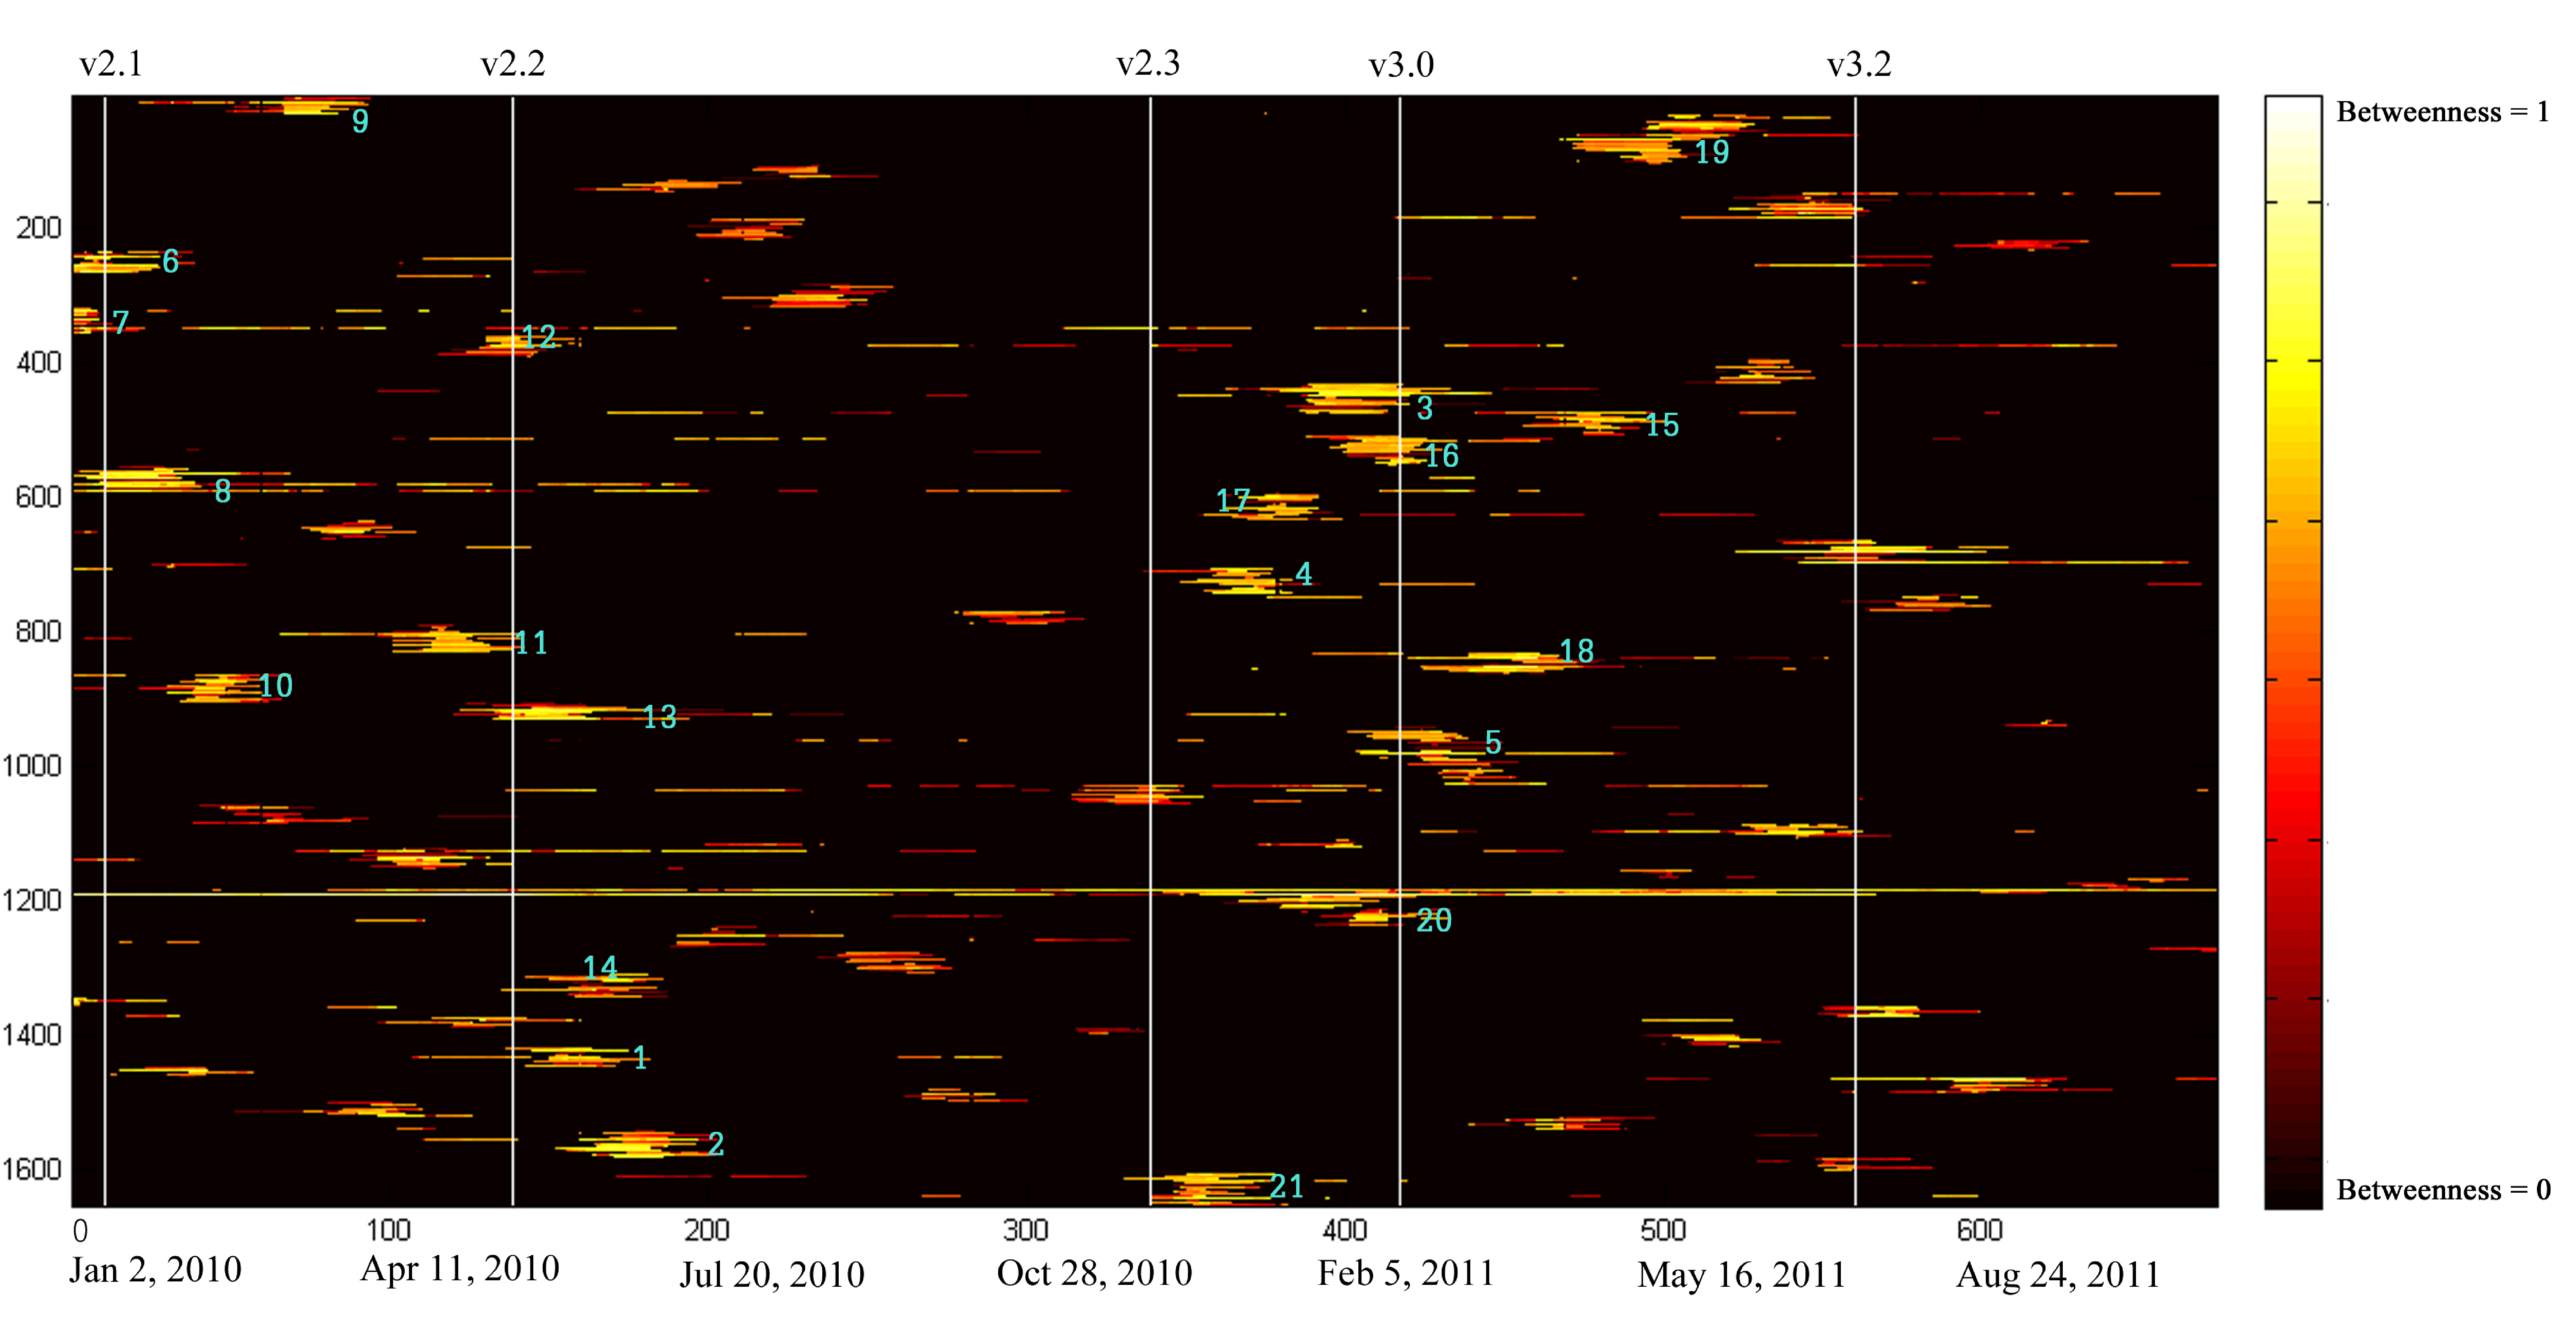
\includegraphics[width=18cm]{result.pdf}
\label{result}
\caption{Betweenness centrality along time line}
\end{figure*}

\section{Results and Analysis}
% describe the figure. 
% take up two columns
\label{results}
We study the results shown in Figure 2. The x-axis represents the number of time windows and the starting dates are denoted every 100 windows. The y-axis represents the number of bug participants who have ever been central in the bug community so that their betweenness centrality values would be greater than 0 for some time period. The color represents the value of betweenness centrality, with darker colors corresponding to lower betweenness and lighter colors for higher betweenness. Each line represents the 673 betweenness centrality values for some bug participant during year 2010 and 2011. In total, we have 1654 bug participants. We clustered the data using K-means with Cosine distance and numbered the participants from 1 to 1654. By studying this result, we made analysis by answering the following questions:

\subsection{Global trend}

\textbf{RQ1. How does the number of active bug participants change over time? Why?}

To give an overview, we compared the interaction of bug participants between 2010 and 2011 along the time line, and found that the interaction among people in Android bug community in 2011 was similar to the interaction of people in 2010 but more frequent. One  \textquotedblleft gap\textquotedblright \ occurs around window 300, which we would explain in the local comparison Section later. 

In addition, correspondingly in Figure 4, the number of active people during 2011 is slightly larger than that of 2010. Also, we can observe that a \textquotedblleft gap\textquotedblright \ around the window 300. Figure 5 shows the sum of betweenness values along the two years' time line, we can see that the trend is very similar to that of the number of active people in Figure 4. This suggests that with more people participating in bug reporting community, the interaction among them increases accordingly.

The reason for the changes of the number of active bug participants and the betweenness centrality values is that around major or minor releases of SDKs, API fixes or improvements, people would become more active taking part in bug reporting, discussing and fixing activities. Also, during these time periods, bugs are more likely to be discovered and reported. Because with the product release pressure, developers would probably work longer and harder than usual with more effort and passion, which promotes the discovery of more bugs and problems of the project. And when the release date is approaching, they have to work hard to fix these bugs. On the other hand, after the release, tremendous users also take part in the activity of discovering the bugs and problems so that in this case both users and developers would like to discuss the bugs. The bug community becomes lively. 

\textbf{RQ2. How does the betweenness centrality of a participant change over time? What are the reasons if they have a certain activity pattern?}

Observing the continuity of betweenness centrality in Figure 3, some people have kept active during the entire two years, and correspondingly they have a very continuous highlighted line. For participants of this type, there are possible explanations. 

First, we suspect these people to be professional developers who belong to the core development team so that what they reported are more important issues which attract more people to discuss and fix them. 

Second, they are probably of high community status or expertises who supervise and guide the development and improvement of the project. They would like to report big issues and will give expertized comments on bugs. 

However, in most cases, participants' betweenness values are distributed dispersedly, as observed in Figure 3. We counted the number of occurrences of the continuous betweenness values which are greater than 0. It means that we would count 1 if the betweenness value is greater than 0 for the first time and take the next values together as the first continuous occurrence until we meet 0. Then the second time we meet value greater than 0, we would count 2 and take the next values together as the second continuous occurrence until another 0 occurs. Except participants who keep active all the time, those with count number 1 would be considered as participants who only appear once. We suspect them to be users. Participants with count number greater than 1 would be phasers who periodically occur in bug community. These randomly phasing participants are very likely to acquire less knowledge or have lower community status in their community, compared to those with continuous high centrality. They might be interested in limited topics and only central and active during the appearance of bugs relevant to those topics.

These possibilities would be validated in Section \ref{validation}.

\subsection{Local Comparison}
\label{local}

\textbf{RQ3. Are there special time ranges that participants are more/less active or central than normal? Why?}

By manually inspecting Android version history, we found that the v2.1 SDK was released on 12 Jan. 2010, which corresponds to the first peak value in Figure 5. v2.2 SDK was released on 20 May 2010 and this corresponds to peak 2. From Dec. 2010 to the beginning of Mar. 2011, several minor updates were released and on 22 Feb. 2011, one major update v3.0 SDK was released. These releases explain the summit, i.e., peak 3, in the figure. That is, there would be more participants discussing and fixing bugs around either major or minor releases, which also indicates that the whole social network is more active around these periods.

In addition, for the first obvious  \textquotedblleft gap\textquotedblright, which covers the time from Oct. 2010 to the end of 2010 (around window 300), there were fewer releases. Social network during this time period is less active and even \textquotedblleft quiet\textquotedblright.

The other bottom value showing up in the end of Figure 5 results from the fact that there are no bug reports recorded in the given dataset and the betweenness value is simply calculated by the comments belonging to bug reports several weeks or months before. 

\textbf{RQ4. What are the possible scenarios for a very sharp change of the participants' centrality?}

Considering individual participants, almost all of them has experienced centrality oscillations. In addition, some groups of people tend to become active and core members during the same time period and then they fade away together. We call them phasers, who phase into centrality and later out of it.

We suspect that the phasers tend to be interested in one or several categories of problems so that they occur only along with the occurrence of these issues. They take part in activities related to the bugs or technical issues and become inactive after the problems solved. Also, by observing the clustered participants of their activity patterns in Figure 3, we suspect that the phasers that show up densely together could be interested in similar categories of topics. This assumption would be validated in Section \ref{validation}. 

\begin{figure}[!t]
\centerline{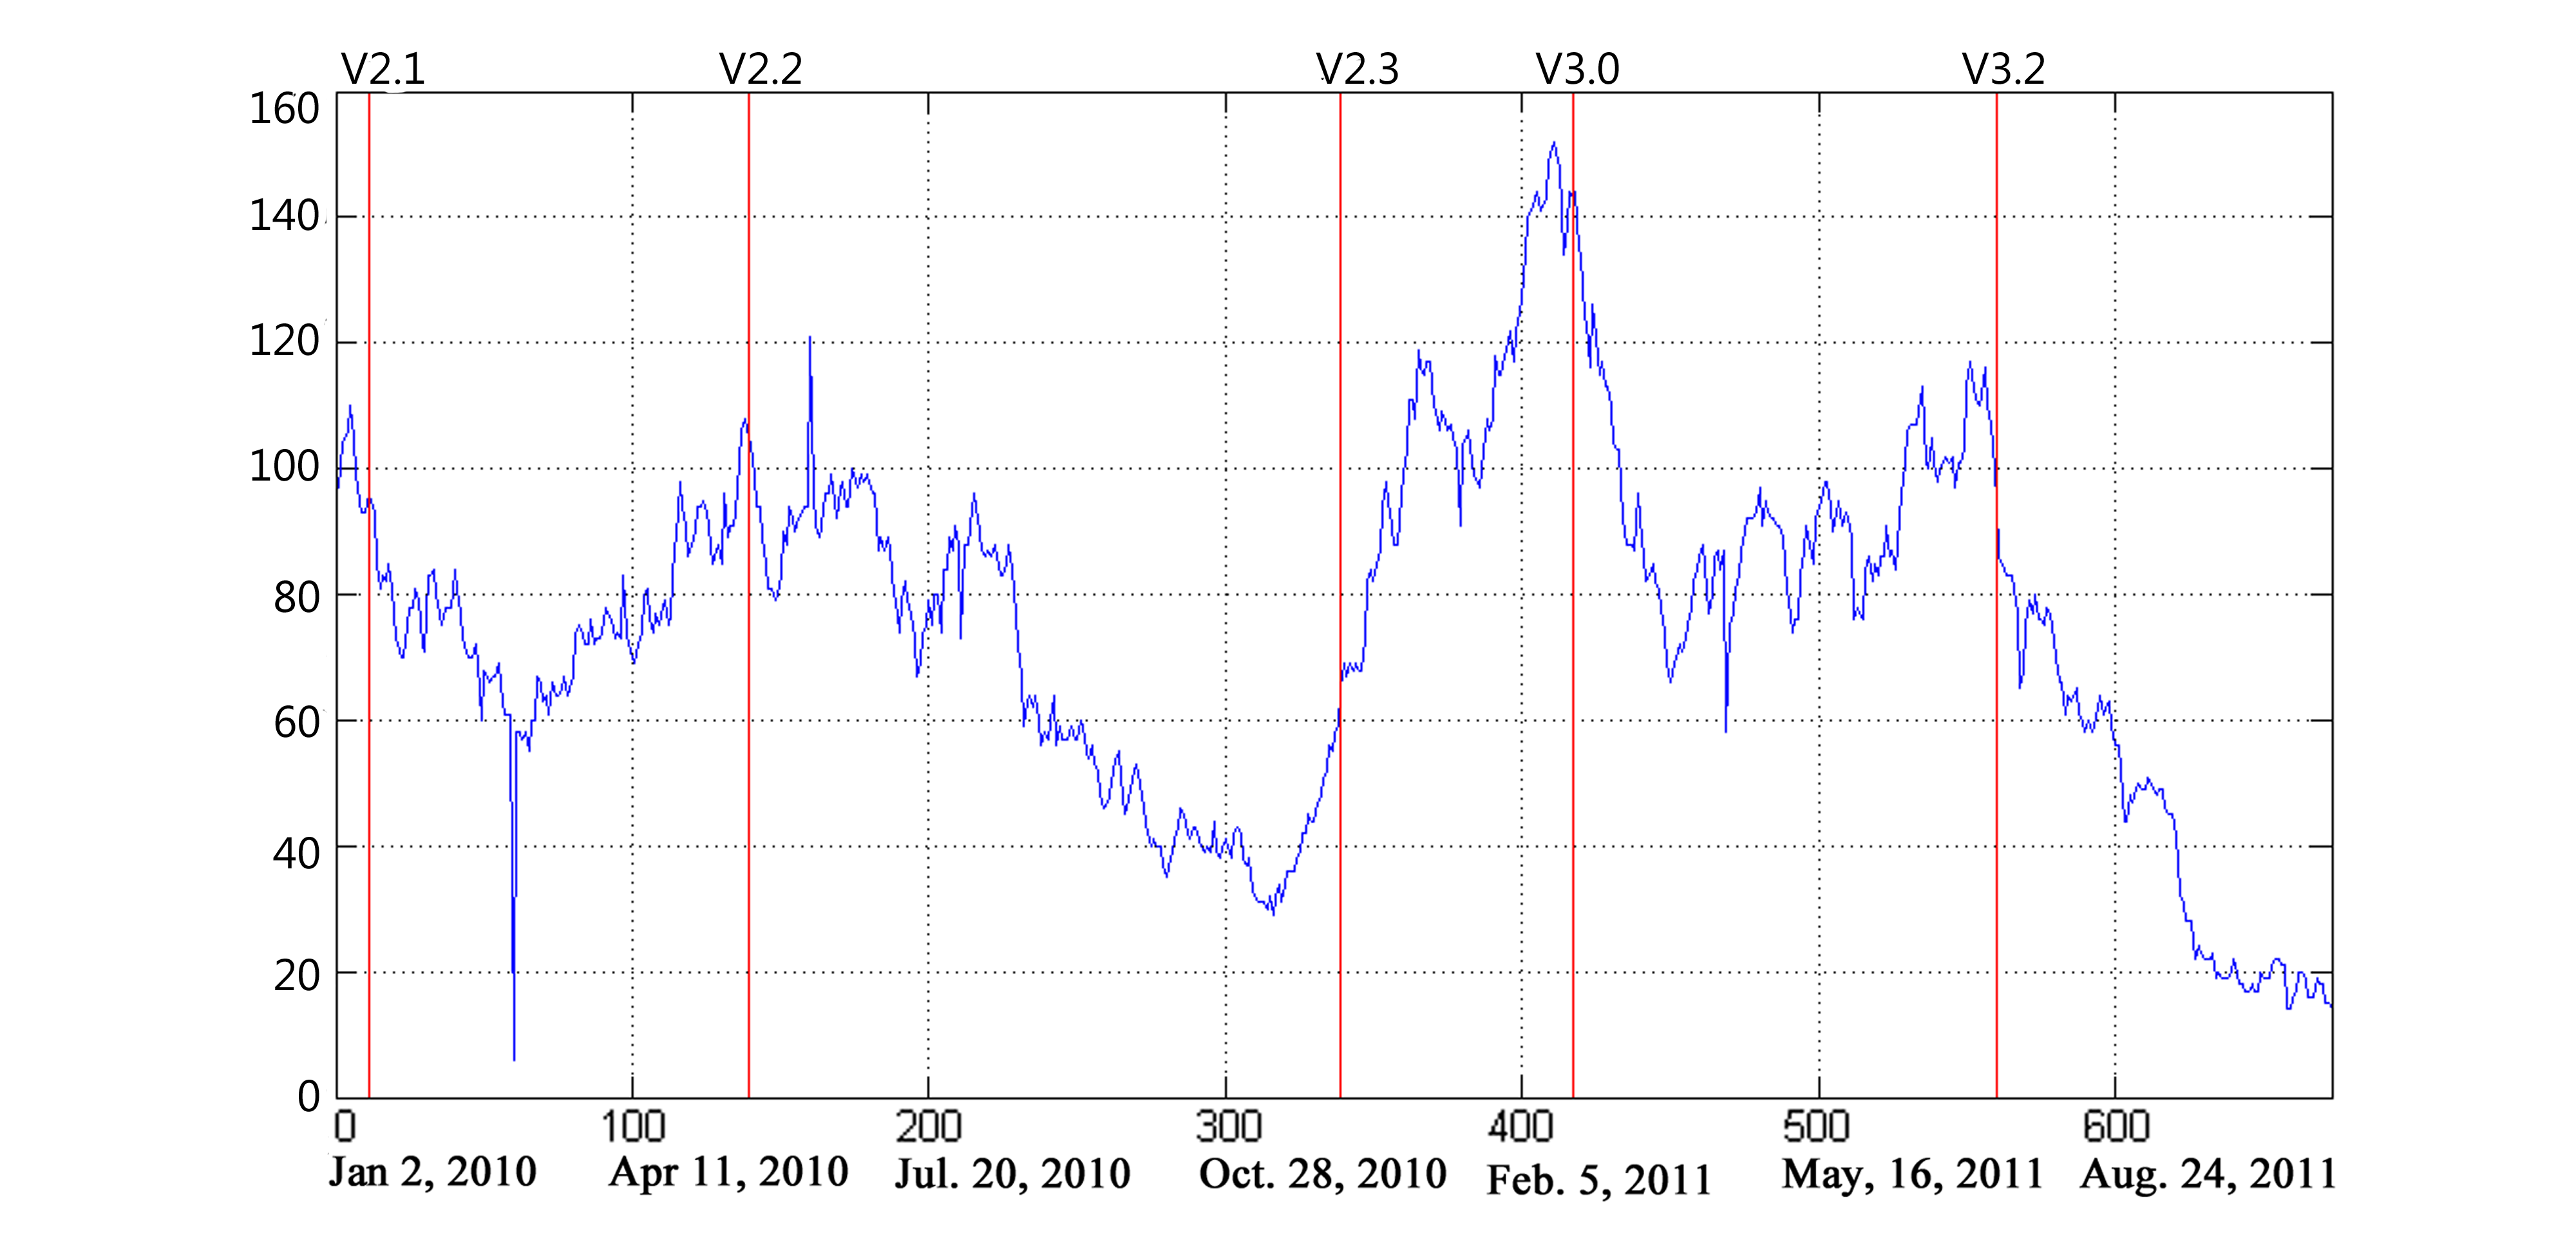
\includegraphics[width=4.1in, height = 4.3cm]{people.png}
\label{people}}
\caption{Number of active people along time line}
\end{figure}

\begin{figure}[!t]
\centerline{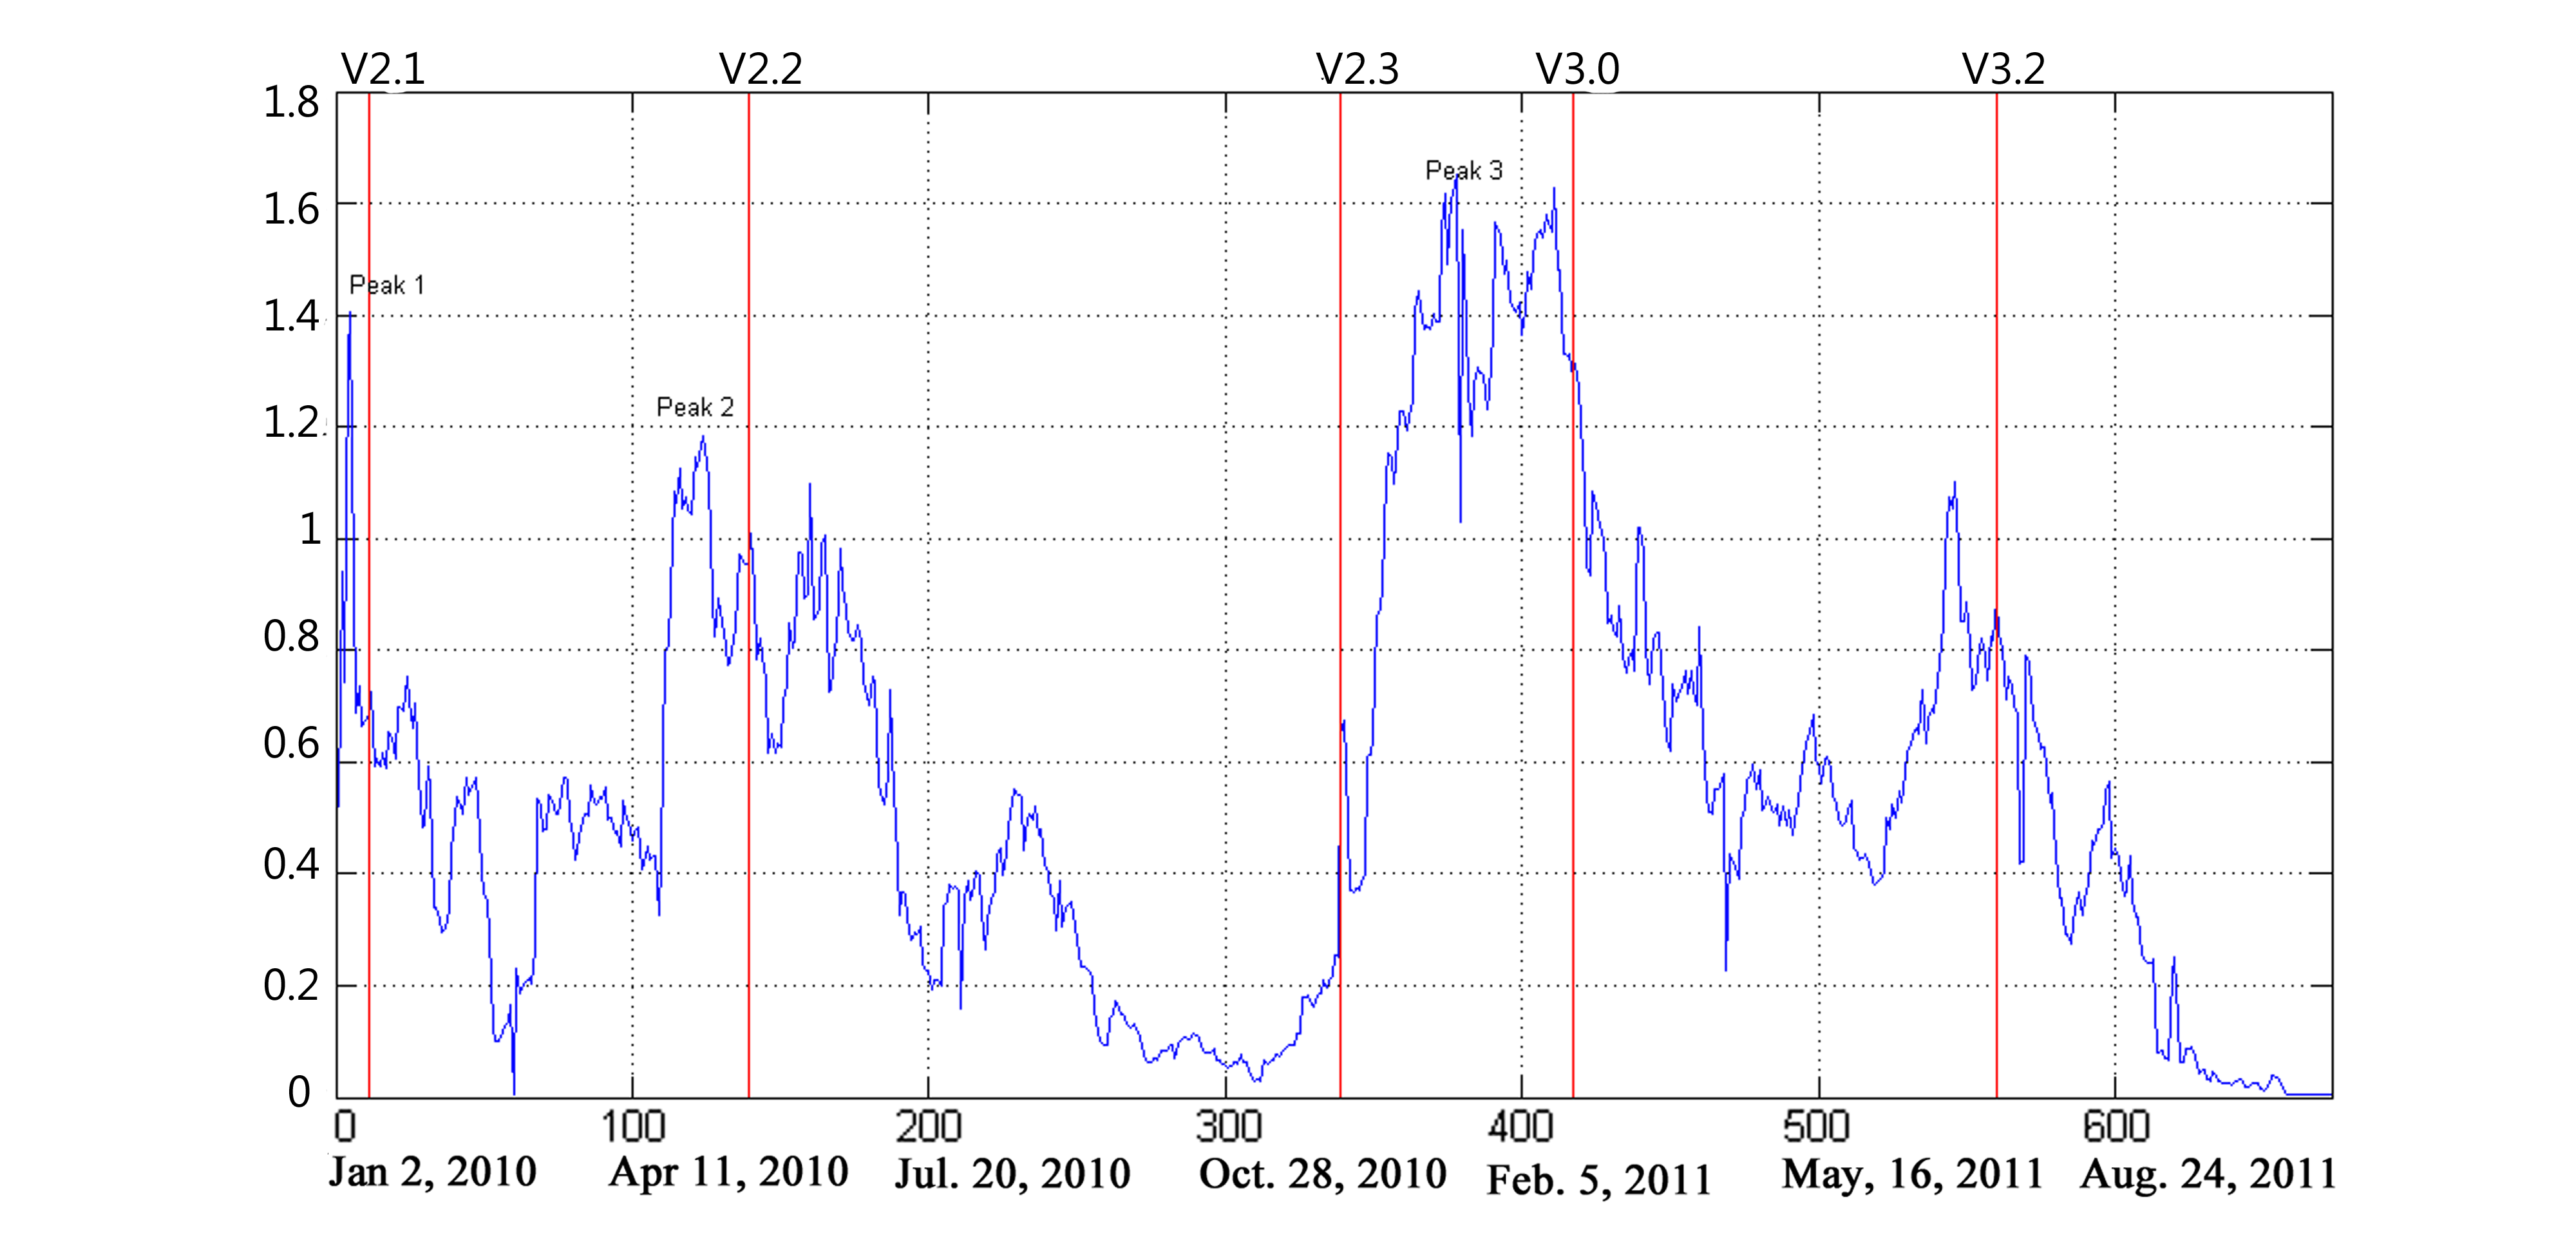
\includegraphics[width=4.1in, height = 4.3cm]{betweenness.png}
\label{betweenness}}
\caption{Sum of betweenness value along time line}
\end{figure}

Meanwhile, other possible explanations for the very sharp change in the participants' centrality could be: 1) the participants are pure users; they showed up merely to report bugs they found. These bugs attract other users or developers to take part in the discussion, which would increase the betweenness centrality of the bug reporters, i.e., the users, for a very short time period. 2) The participants are developers and they left their jobs temporarily, for a vacation for example. Besides, they could also leave their jobs permanently because of retiring or working for another project. 3) The project is just finished or discarded so that both users and developers would not discuss anything about it any more. This group of people could be verified by looking for those who do not own any submission and then regarded as pure users. The third explanation would be easily substantiated by inspecting Android version release history. However, the second explanation is hard or even impossible to validate with the very limited information we could get from the repositories and the release history. Participants should be contacted in person for such validation, which has not been done in our study.



\section{Validation}
\label{validation}
% This section needs to be modified!!!
% two parts: 1. assumption, take up 2 columns 2. validation, take up 3 columns
% validation: 1. clusters 2. phasers
\subsection{Activity pattern validation}
Among the 1654 participants with betweenness values larger than 0, we analyzed their centrality patterns and divide them into three categories: 
1) participants appeared only once, with a number of 71 out of 1654 participants (we are not considering those eliminated participants with betweenness values equal to 0, these eliminated participants actually count up to a number of 30969 - 1654 = 29315), 
2) participants recurred periodically, with a number of 1575 participants,
and 3) participants who are central along the entire time line, with a number of 8 participants.

From the mining results, we notice that there is a small group of people who have been central for almost all the time; another relatively larger group appear without any recurrence; the majority would periodically become central in their community. Based on the three activity patterns, we have found some interesting discoveries as following:

\subsubsection{Participants appeared only once tend to be pure users}
We look into the Android changes repository to find the files submitted by the 71 participants who have appeared only once in the bug community. We find that 7 of them have ever submitted a change, which means that they probably are developers other than pure Android users. However, these 7 participants only take up 10\% of the total 71 participants and most of them have never submit anything to the development community. This verifies our assumption that participants appeared only once in the bug community would more likely be pure users.

\subsubsection{Participants showed up periodically should be a combination of users and developers}
Periodically appearing participants are the majority and they are called phasers. We sampled 4 continuous portions of them (continuous means they are continuously numbered in the clustered results): participants 430 to 474, 704 to 742, 1418 to 1447, and 1543 to 1584. For each of the four groups, the number of developers are 5, 13, 9, 7 respectively. They take up 17\%, 32\%, 20\%, and 18\% of the total number of participants in each group. 

Further, we studied the specialties of the developer participants from the four sampled groups. All except two of them have worked on tasks related with specific techniques so that they are actually specialized in some topics. 

The rest of the periodically appearing participants have never submitted files to the development community. They are probably users of Android. Thus, phasers consist of both users and developers. Developers of this group are usually interested in some specific topics.

\begin{table}[!t]
%% increase table row spacing, adjust to taste
% if using array.sty, it might be a good idea to tweak the value of
% \extrarowheight as needed to properly center the text within the cells
\caption{5 continuously central participants who have submissions in the changes repository. On the forth row, ralf and Ralf.Hildebrandt are email alias of the same person, as we observed that the author\_name attributes are the same for the two email alias.}
\label{continuous_project}
\centering
%% Some packages, such as MDW tools, offer better commands for making tables
%% than the plain LaTeX2e tabular which is used here.
\begin{tabular}{|p{1.2cm}|p{1.1cm}|p{4.6cm}|}
\hline
Participant & \#Submitted-\_changes & Related Project \\
\hline
fadden & 1259 & device\_samsung\_crespo, platform(bionic, build, dalvik, etc.) \\
\hline
xav & 3501 & platform(frameworks\_base, build, external\_bouncycastle, etc.), device\_sample, \\
\hline
mbligh & 80 & kernel(common, experimental, linux-2.6, msm, omap, qemu, samsung, tegra) \\
\hline
ralf (Ralf.-Hildebrandt) & 665 & kernel(common, experimental, linux-2.6, dalvik, external\_libpng, sdk,system\_core, etc.) \\
\hline
romainguy & 1455 & device\_htc\_passion, device\_samsung\_crespo, platform(build, cts, dalvik, development, external\_bouncycastle, libcore, ndk, apps(AccountsAndSyncSettings, AlarmClock,
Bluetooth, Browser, Calculator, etc.),
inputmethods(LatinIME, iOpenWnn, PinyinIME, CalendarProvider),
providers(DownloadProvider, GoogleSubscribedFeedsProvider), wallpapers(Basic, LivePicker,
MagicSmoke, MusicVisualization), prebuilt, sdk, system\_core) \\
\hline
\end{tabular}
\end{table}


\subsubsection{Participants who were continuously central could have multiple specialties}
5 out of the 8 participants in this group have submissions in the changes repository and they take up to 62.5\%, which is significantly larger than the previous two groups.

We extracted the projects these 5 participants have submitted changes to, as listed in Table \ref{continuous_project}.

Firstly, considering the number of changes they made, all of them except mblign have submitted more than 500 files to the changes repository, which means that they are quite active in Android development community. This could to some extent prove that they are experts or advanced developers since more submissions usually represent broader knowledge about the related techniques, especially in such volunteered open source development community.

Moreover, fadden, xav, and romainguy are all working on the platform, which includes build, dalvik, development, framework base, libcore, sdk, etc. All of their specialties are related to the platform or system core aspects, and should be important along the entire development. In this case, continuously central participants should have experiences on the system core related topics. This is an interesting point beyond our hypothesis.

Further, the participant romainguy has experiences on almost every part related to platforms, including both the apps and the core, and hence should be considered as Android platform development leader.

To summarize, three different centrality patterns correspond to participants of three categories, which proves our analysis hypothesis in Section \ref{results}.

\begin{table}[!t]
\centering
\caption{5 clusters we have chosen, out of a total number of 21.}
\begin{tabular}{|c|c|}
\hline
Cluster & Time  \\
\hline
1 & May 16, 2010 - Jun. 24, 2010 \\
\hline
2 & Jun. 2, 2010 - Jul. 24, 2010  \\
\hline
3 & Jan. 13, 2011 - Mar. 3, 2011 \\
\hline
4 & Dec. 3, 2010 - Jan. 31, 2010 \\
\hline
5 & Feb. 4, 2011 - May 1, 2011 \\
\hline
\end{tabular}
\label{cluster_list}
\end{table}

\begin{table}[!t]
%% increase table row spacing, adjust to taste
\renewcommand{\arraystretch}{1.3}
% if using array.sty, it might be a good idea to tweak the value of
% \extrarowheight as needed to properly center the text within the cells
\caption{Participants and their specialties in cluster No. 4}
\label{cluster_no4}
\centering
%% Some packages, such as MDW tools, offer better commands for making tables
%% than the plain LaTeX2e tabular which is used here.
\begin{tabular}{|c|c|c|}
\hline
ID & Name & Specialties \\
\hline
1 & Charles Chin & kernel - sound, kernel\_linux-2.6 \\
\hline
2 & Josh Guilfoyle & ringtone, media \\
\hline
3 & Kristoffer Ericson & driver(net, video, serial, input) \\
\hline
4 & Rik Bobbaers & kernel\_linux-2.6(mlock) \\
\hline
5 & Rikard Olsson & kernel\_linux-2.6(arm) \\
\hline
6 & Riku Voipio & kernel\_linux-2.6(arm), driver \\
\hline
7 & Haris Peco & platform sdk(eclipse plugin) \\
\hline
\end{tabular}
\end{table}

\begin{table*}[!t]
%% increase table row spacing, adjust to taste
% if using array.sty, it might be a good idea to tweak the value of
% \extrarowheight as needed to properly center the text within the cells
\caption{Participants' common specialties of each cluster. Participants number is counted as the number of participants within each cluster who has ever submitted a change and appeared in the change repository, ie., developers.}
\label{cluster_topic}
\centering
%% Some packages, such as MDW tools, offer better commands for making tables
%% than the plain LaTeX2e tabular which is used here.
\begin{tabular}{|c|c|c|}
\hline
Cluster & Participants Number & Specialties \\
\hline
1 & 5 & netfilter, driver(video), tests, MIPS \\
\hline
2 & 13 & driver(usb, wireless, mouse), sound, net, i386, performance(tools), input methods \\
\hline
3 & 9 & sound, driver, frameworks\_base, tests, platform, kernel \\
\hline
4 & 7 & sound, media, kernel\_linux-2.6, driver, platform sdk, kernel video/serial \\
\hline
5 & 63 & net(bluethooth, net driver, ipv$x$, kernel\_linux-2.6), driver(dvd, media, usb, gpu, net), ia64, sound, tests \\
\hline
\end{tabular}
\end{table*}

\begin{table*}[!t]
%% increase table row spacing, adjust to taste
% if using array.sty, it might be a good idea to tweak the value of
% \extrarowheight as needed to properly center the text within the cells
\caption{Release time and contents, nearby which our chosen clusters are located}
\label{release}
\centering
%% Some packages, such as MDW tools, offer better commands for making tables
%% than the plain LaTeX2e tabular which is used here.
%lp{3in}
\begin{tabular}{|c|c|p{9.5cm}|c|}
\hline
Release & Time & Highlights & Related cluster\\
\hline
v2.2 & May 20, 2010 & camera and gallery, portable wifi, multiple keyword language, performance(general, browser), media framework, Bluetooth, kernel upgrade, APIs(media, camera, graphis, data backup, device administrator, UI framework) & 1 \\
\hline
v2.2.1 & Jan. 18, 2011 & bug fixes(one is about root and unroot), security updates, performance improvements & 3\\
\hline
v2.2.2 & Jan. 22, 2011 & fixed minor bugs, including SMS routing issues & 3\\
\hline
v2.3 & Dec. 6, 2010 & UI refinements, faster text input, power management, NFC, multiple cameras, download management, new multimedia, new developer features(gaming, communication, multimedia, garbage collector, event distribution, video driver, input, native access-audio, graphics, storage, development), linux kernel upgrade to 2.6.36, Dalvik runtime, mixable audio effects & 4\\
\hline
v2.3.3 & Feb. 9, 2011 & NFC, Bluetooth, Graphics, media, framework, speech recognition, voice search, API(identifier, build-in app, locales), emulator skins & 5 \\
\hline
v3.0 & Feb. 22, 2011 & UI design for tables, redesigned keyboard, improved text selection, copy and pase, connectivity options(USB, WIFI, media, keyboard, bluetooth), apps update, browser, camera and gallery, contacts, email, development support & 5 \\
\hline
\end{tabular}
\end{table*}




\subsection{Cluster validation}

As we have discussed above, participants are more active around important releases. Moreover, we can observe from Figure 3 that participants' centrality distributions tend to form into groups, which locate around the release point, i.e., when participants are clustered according to their centrality values, they form into groups. Participants belonging to the same group become central during the same time periods and then fade away together.

We denoted 21 visible clusters from Figure 3 and looked into five of them. 
The five clusters we chose are listed in Table \ref{cluster_list}

We extract changes submitted by the members of each cluster from the Android changes repository. (For those who do not have records in the changes repository, we regard them as pure users and do not consider them in this case). After inspecting their submissions, we would get an idea about what kind of tasks they have been mostly working on.
We take both the release history and the change submission records as the fact in reality, and we find our hypothesis in Section \ref{results} matched with the reality we got here. 

We have found the following facts that prove our hypothesis:

\subsubsection{Participants clustered together share similar specialties and tasks}

Our analysis in Section \ref{results} shows that the phasers that show up densely together could be interested in similar categories of topics or working on tasks related to the same area.

As described in Section \ref{methodology}, we extract the targets and project names from the changes repository for each member appeared within the cluster. The specialties could be inferred by the contents of the targets and the topics of the projects. Specialties of clusters are summarized in Table \ref{cluster_topic}:

% An example of a floating table. Note that, for IEEE style tables, the 
% \caption command should come BEFORE the table. Table text will default to
% \footnotesize as IEEE normally uses this smaller font for tables.
% The \label must come after \caption as always.

Inspecting the specialties, we find that each cluster has their own topics, which are relatively different from others'. Also, topics of each cluster are concentrated on a limited specific technique areas. For example, cluster No.1 covers techniques about net filters, drivers, tests, and MIPS, while cluster No.2 is about drivers for connecting devices (usb, wireless, and mouse), net, processor, and input. It is easy to tell that participants of these two clusters are working on different tasks. The other clusters could lead to the same conclusion. This concludes that each cluster has its own participants-shared specialties.

Further, if we look into one of the clusters, we can see that sub-groups exist in each cluster, and each sub-group works on one common topic. Take cluster No.4 as an example. There are 7 developers contained in this cluster, as listed in Table \ref{cluster_no4}.

It can be obviously observed that work of participants in this cluster could be generally divided into two groups: one is about the linux 2.6 based kernel, another is on stuffs related to media. Charles Chin, Rik Bobbaers, Rikard Olsson, and Riku Voipio are all doing the linux 2.6 kernel. Charles Chin, Josh Guilfoyle, and Kristoffer are working on the media, which actually includes sound, video drivers, or ringtone. Besides, we even guess that these two specialties may have strong connection so that those who work on the kernel are likely to work on the media related part. For example, the projects Charles Chin is working on are all about the kernel, with sound as the target, which means he is working on the sound related kernel, and it is the same with Kristoffer.

If we look into other clusters, we can make the same conclusions.
Thus, from the observation and analysis above, we can conclude that participants with similar centrality patterns share similar specialties and tasks.

\subsubsection{Clusters' working specialties are in accordance with the release contents along the time line}

When observing the Android release history, we have made conclusion that the overall betweenness centrality becomes higher when there are releases, and more active participants appear around important releases, according to Figure 4 and Figure 5.

In addition, when taking participants' specialties into consideration, we find that the release contents are in accordance with the specialties for members of each cluster. Table \ref{release} lists releases and their corresponding clusters together with the highlighted working contents.

Comparing the release contents and the cluster specialties, these two subjects are mostly matched on release topics and cluster's working contents. For example, cluster No.4 covers from December 3, 2010 to January 31, 2011, which locates before release v2.3. Participants in cluster No.4 have specialties on sound, media, and kernel-video, which match the release contents of new multimedia, APIs for native audio, and mixable audio effects in v2.3; specialties about driver on video, input and keyboard match the contents featured on video driver and the faster text input accordingly. We can also find that 4 out of 7 developers in cluster No.4 has worked on kernel 2.6, which corresponds to the linux kernel upgraded to 2.6.36 in v2.3.
For cluster No.3, which ranges from January 13, 2011 to March 3, 2011, during which time v2.2.1 and v2.2.2 are released on January 18, 2011 and January 22, 2011 respectively. Release 2.2.1 contains security updates and performance improvement, which should focus on the bottom layer; at the same time, participants in cluster No.3 are specialized mostly on kernels or platforms. These two facts are thus in accordance. This phenomenon happens in cluster No.1 and its corresponding release v2.2 as well.

Therefore, the conclusion is that participants' working specialties within clusters are in accordance with the related release contents along the time line.
% An example of a floating figure using the graphicx package.
% Note that \label must occur AFTER (or within) \caption.
% For figures, \caption should occur after the \includegraphics.
% Note that IEEEtran v1.7 and later has special internal code that
% is designed to preserve the operation of \label within \caption
% even when the captionsoff option is in effect. However, because
% of issues like this, it may be the safest practice to put all your
% \label just after \caption rather than within \caption{}.
%
% Reminder: the "draftcls" or "draftclsnofoot", not "draft", class
% option should be used if it is desired that the figures are to be
% displayed while in draft mode.
%
%\begin{figure}[!t]
%\centering
%\includegraphics[width=2.5in]{myfigure}
% where an .eps filename suffix will be assumed under latex, 
% and a .pdf suffix will be assumed for pdflatex; or what has been declared
% via \DeclareGraphicsExtensions.
%\caption{Simulation Results}
%\label{fig_sim}
%\end{figure}

% Note that IEEE typically puts floats only at the top, even when this
% results in a large percentage of a column being occupied by floats.


% An example of a double column floating figure using two subfigures.
% (The subfig.sty package must be loaded for this to work.)
% The subfigure \label commands are set within each subfloat command, the
% \label for the overall figure must come after \caption.
% \hfil must be used as a separator to get equal spacing.
% The subfigure.sty package works much the same way, except \subfigure is
% used instead of \subfloat.
%
%\begin{figure*}[!t]
%\centerline{\subfloat[Case I]\includegraphics[width=2.5in]{subfigcase1}%
%\label{fig_first_case}}
%\hfil
%\subfloat[Case II]{\includegraphics[width=2.5in]{subfigcase2}%
%\label{fig_second_case}}}
%\caption{Simulation results}
%\label{fig_sim}
%\end{figure*}
%
% Note that often IEEE papers with subfigures do not employ subfigure
% captions (using the optional argument to \subfloat), but instead will
% reference/describe all of them (a), (b), etc., within the main caption.




% Note that IEEE does not put floats in the very first column - or typically
% anywhere on the first page for that matter. Also, in-text middle ("here")
% positioning is not used. Most IEEE journals/conferences use top floats
% exclusively. Note that, LaTeX2e, unlike IEEE journals/conferences, places
% footnotes above bottom floats. This can be corrected via the \fnbelowfloat
% command of the stfloats package.

\section{Limitations}
% take up 1 column
\label{limitation}
In this study we explicitly trust that the same account of email addresses, i.e., the part before \textquotedblleft @\textquotedblright, belongs to the same bug participant. With the given semi-anonymous email addresses in Android bug repository, we pruned the part starting from \textquotedblleft ....\textquotedblright  and kept the front part as the names of bug participants. However, it is possible that some common names share the same start string. For example, \textquotedblleft Benjamin Franzke\textquotedblright, \textquotedblleft Benjamin Tissoires\textquotedblright  and \textquotedblleft Benjamin Romer\textquotedblright  have the same first name. We cannot distinguish these names with the email address \textquotedblleft Benjamin@XXX'. Besides, some of the email addresses start with a simple letter which is ambiguous identifying a person, while we analyze the results without excluding such data.

In addition, among the 1654 bug participants whose betweenness centrality has ever been larger than 0, more than 1500 of them are periodically appearing participants. We sampled 4 groups of people since the results from these sampled data are representative to substantiate the assumption we have made for periodically appearing participants.

We analyze the results based on another assumption that the types of submitted files reflect the techniques the developers are specialized in. Hence, we tagged the participants with the techniques according to their submitted files in the Android changes repository. However, there could exists inconsistency to some extend between the techniques and the submitted files. 

\section{Conclusion and Future Work}
% take up 1 column
\label{conclusion}
In this paper, we mined the Android bug repository and studied the data of 2010 and 2011. We used an overlapping time windowing technique and applied social network analysis to analyze the bug reports community. 

We did our analysis by answering four questions about the temporal evolution of Android bug reporting community, on view of both globally and locally. Moreover, after manually inspecting Android version history, we found answers to explain sharp changes and occurrences of specific time ranges. Most minor or major releases lead to high betweenness centrality in general. With the data from Android changes repository, we further validated the three activity patterns of bug participants and find reasons for their being clustered. Participants who have high betweenness centrality at the same time period show interest in the same topics and acquire related techniques.

Future work includes applying the approach in this paper to other open source projects' repository, so as to expect whether results from our overlapping time windowing SNA are trustworthy enough to reflect facts in the actual developing process. 



% conference papers do not normally have an appendix


% use section* for acknowledgement



% trigger a \newpage just before the given reference
% number - used to balance the columns on the last page
% adjust value as needed - may need to be readjusted if
% the document is modified later
%\IEEEtriggeratref{8}
% The "triggered" command can be changed if desired:
%\IEEEtriggercmd{\enlargethispage{-5in}}

% Better way for balancing the last page:

\balance

% references section

% can use a bibliography generated by BibTeX as a .bbl file
% BibTeX documentation can be easily obtained at:
% http://www.ctan.org/tex-archive/biblio/bibtex/contrib/doc/
% The IEEEtran BibTeX style support page is at:
% http://www.michaelshell.org/tex/ieeetran/bibtex/
%\bibliographystyle{IEEEtran}
% argument is your BibTeX string definitions and bibliography database(s)
%\bibliography{IEEEabrv,../bib/paper}
%
% <OR> manually copy in the resultant .bbl file
% set second argument of \begin to the number of references
% (used to reserve space for the reference number labels box)
\begin{thebibliography}{2}


\bibitem{ICSMwindowed:hindle}
A. ~Hindle, M.W. Godfrey, and R.C. Holt, \emph{What's hot and what's not: Windowed developer topic analysis}, \hskip 1em plus
  0.5em minus 0.4em \relax  IEEE International Conference on Software Maintenance, 2009. ICSM 2009

\bibitem{ICSEsocio:meneely}
A. ~Meneely and L. ~Williams. Daly, \emph{Socio-Technical Developer Networks: Should we Trust Our Measurements?}, \hskip 1em plus
  0.5em minus 0.4em\relax Honolulu, Hawii, USA, ICSE'11 May 21-28, 2011
  
 \bibitem{ICSEsocio:la}
U. ~Brandes and T. ~Erlebach, \emph{Network Analysis: Methodological Foundations}, \hskip 1em plus
  0.5em minus 0.4em\relax Berlin, Springer, 2005

\bibitem{Springer:kidane}
Y. ~Kidane and P. ~Gloor, \emph{Correlating temporal communication patterns of the Eclipse open source community with performance and creativity
}, \hskip 1em plus
  0.5em minus 0.4em\relax Springer, 2007

\bibitem{Procedia:ibaa}
T. ~Ibaa, K. ~Nemotob, B. ~Petersc, P. ~Gloor, \emph{Analyzing the Creative Editing Behavior of Wikipedia Editors: Through Dynamic Social Network Analysis}, \hskip 1em plus
  0.5em minus 0.4em\relax Procedia - Social and Behavioral Sciences, 2 (4), pp. 6441-6456, 2010

\bibitem{AMCIS:Freeh}
V. ~Freeh, R. ~Tynan, G. ~Madey, \emph{Applying social network theory}, \hskip 1em plus
  0.5em minus 0.4em\relax Dallas, TX, USA, AMCIS, page 1086-1813, 2002

\bibitem{ACM:chris}
C. ~Bird, D. ~Pattison, R. ~D'Souza, V. ~Filkov, and P. ~Devanbu, \emph{Latent social structure in open source projects}, \hskip 1em plus
 0.5em minus 0.4em\relax New York, NY, USA, ACM, 2008

\bibitem{ACM:ashish}
A. ~Sureka, A. ~Goyal, A. ~Rastogi, \emph{Using social network analysis for mining collaboration data in a defect tracking system for risk and vulnerability analysis}, \hskip 1em plus
 0.5em minus 0.4em\relax Thiruvananthapuram, Kerala, India, ACM, 2011

\bibitem{MSR:christ}
C. ~Bird, A. ~Gourley, A. ~Swaminathan\emph{Mining Email Social Networks}, \hskip 1em plus
 0.5em minus 0.4em\relax Shanghai, China, MSR, 2006

\bibitem{OSD:yasu}
Y. ~Kamei, S. ~Matsumoto, H. ~Maeshima, Y. ~Onishi, M. ~Ohira, and K. ~Matsumoto\emph{Analysis of Coordination Between Developers and Users in the Apache Community}, \hskip 1em plus 0.5em minus 0.4em\relax 2008, in IFIP International Federation for Information Processing, Volume 275; Open Source Development, Communities and Quality; Barbara
Russo, Ernesto Damiani, Scott Hissam, Björn Lundell, Giancarlo Succi; (Boston: Springer), pp. 81–92.

\bibitem{BOOK:han}
H. ~Robert A. and M. ~Riddle \emph{Introduction to social network methods}, \hskip 1em plus
 0.5em minus 0.4em\relax Riverside, CA:  University of California, USA, 2005

\bibitem{DATA:msr}
E. ~Shihab and Y. ~Kamei and P. ~Bhattacharya\emph{Mining Challenge 2012: The Android Platform}, \hskip 1em plus
 0.5em minus 0.4em\relax The 9th Working Conference on Mining Software Repositories, to appear, 2012





\end{thebibliography}




% that's all folks
\end{document}


